\documentclass[editMode]{ufdissertation}\sloppy
  \usepackage{tikz}%       tikz is used by almost everyone, but certainly by me for this.
  \usepackage{bm}%         bm is needed in order to boldface mathematical symbols
  %% Uncomment the relevant line below if you have tables or figures.
  \haveTablestrue%        Uncomment this if you have tables in your thesis.
  \haveFigurestrue%       Uncomment this if you have figures in your thesis.
  % \haveObjectstrue%       Uncomment this if you have Objects in your thesis. This is almost certainly not the case however.

  \title{The Implementation of QM/MM on Non-Adiabatic Dynamics Using AMBER and NEXMD}%  Put your title here.

  \degreeType{Doctorate of Philosophy}%   Official name of your degree; eg "Doctorate of Philosophy".
  \major{Mathematics}%                    Your official Department
  \author{Dustin Tracy}%                  Your Name
  \thesisType{Dissertation}%              Dissertation (PhD) or Thesis (Masters)
  \degreeYear{2021}%                      Intended graduation year (not the year you submit the thesis)
  \degreeMonth{May}%                   Month of graduation should be May, August, or December.
  \chair{Adrian Roitberg}%                   Chair and Cochair (see comment block above).


  %%%%%%%%%%%%%%%%%%%%%%%%%%%%%%%%%%%%%%%%%%%%%%%%%%%%%%%%%%%%%%%%%%%%%%%%%%%%%%%% 
%%% For each of the following, type in the name of the file that contains each section. 
%       They are assumed to be tex files, but if they aren't the command takes an optional argument for the extension.
%       So, you could load dedication.tex as your dedication file using \setDedicationFile{dedication}
%       You could load dedication.txt instead with \setDedicationFile[txt]{dedication}.
%       NOTE: For some compilers they may or may not add a .tex to the end of the file automatically.
%           If you get a "couldn't find dedication.tex.tex" type error, try the command with an empty optional argument,
%           e.g. \setDedicationFile[]{dedication}
%%%
%%%%%%%%%%%%%%%%%%%%%%%%%%%%%%%%%%%%%%%%%%%%%%%%%%%%%%%%%%%%%%%%%%%%%%%%%%%%%%%%

%%% These are REQUIRED sections; easiest to do via these commands.

\setDedicationFile{dedicationFile}%                 Dedication Page
\setAcknowledgementsFile{acknowledgementsFile}%     Acknowledgements Page
\setAbstractFile{abstractFile}%                     Abstract Page (This should only include the abstract itself)
\setReferenceFile{referenceFile}{amsplain}%         References. First argument is your bibtex source file
%                                                       the second argument is your bibtex style file.
\setBiographicalFile{biographyFile}%                Biography file of the Author (you).

%%% These are NOT required, so only use them if you actually need/have them.

% \setAbbreviationsFile{abbreviations}%           Abbreviations Page
% \setAppendixFile{appendix}%                     Appendix Content; hyperlinking might be weird.
% \multipleAppendixtrue%                          Uncomment this if you have more than one appendix, 
%                                                   comment it if you have only one appendix.


%%%%%%%                     End of File Assignment
%%%%%%%%%%%%%%%%%%%%%%%%%%%%%%%%%%%%%%%%%%%%%%%%%%%%%%%%%%%%%%%%%%%%%%%%%%%%%%%%

\begin{document}
%%%% Here you just need to include/input your actual work. 
%       The above files (dedication, acknowledgement, titlepage, etc etc) will all be added for you 
%       using the files you assigned above. 
%       If you want to input the above files manually you can comment out the \setFILE command above 
%       and use \input or \include here. Generally you want to use \include to get your pagebreak.
%       NOTE: If you input manually you will have to do some/all the formatting manually.



\chapter{Introduction} \label{introduction}

\section{Prologue}

The effects of light on materials' physical properties have maintained humanity's interest for as long as history itself. Humans most likely noticed the power of the sun to turn their skin red and itchy far before they even developed language. Records show an interest in reducing the bleaching dyes, for example.\cite{roth1989beginnings} The documents describing Archimedes' mirror demonstrate that human's desire to harness this power dates back at least multiple millennia.\cite{claus1973archimedes} Our understanding began to formalized in the late 1700s when Priestly experiments shined a light on the oxidation processes and sparked a curiosity that led to further experimentations with photosynthesis and photochemistry in general.\cite{priestley1772observations} Since then, researchers have further advanced our knowledge of these effects and our ability to harness the power of light.

The ability to model these photo-energetic non-adiabatic dynamics has recently become more feasible.
We have used this ability to continue our long pursuit to understand organic photosynthesis and search for efficiently creating and utilizing synthetic organic photosynthesis. \cite{zheng2017photoinduced,caycedo2010light,balzani2008photochemical,engel2007evidence}
Recent capabilities to simulate these dynamics with computers have helped determine the feasibility of prospective light-harvesting technologies. \cite{ishida11_effic_excit_energ_trans_react,katan2005effects}

This type of modeling can also help with understanding photo-detection.
Recent works, for example, have helped understand how the photo-detecting protein rhodopsin behaves in the human eye.\cite{weingart2012modelling}
Continued research is expected to develop more sensitive or energy-efficient optical sensors. 

Certain classes of organic conjugated molecules possess characteristics that make them the prototypical choice to develop highly efficient light-emitting diodes (LEDs). 
The modeling of these molecules' photochemical dynamics currently boasts a broad academic and industrial interest. \cite{tavernelli2010nonadiabatic,tavernelli2015nonadiabatic,nelson2020non}
The photophysical characteristics of these molecules change significantly in the presence of solvents.
An immense amount of improvements to simulates this behavior have been made in just that last decade alone. This paper aims to provide an additional tool to help further illuminate these understanding.

\section{Qualitative Overview of Non-Adiabatic Dynamics}

\subsection{Energy Transfer}

\noindent
	  \begin{multiFigure} 
	    \addFigure{0.45}{../Oral/Images/photoexcitation.png}
	    \addFigure{0.45}{../Oral/Images/pes_chart_zoomed.png}
	    \captionof{figure}{Diagrams describing the behavior of a molecule throughout a photo-excitation event.}
	    \label{fig:jablonski}
	  \end{multiFigure}
\bigskip

Figure \ref{fig:jablonski} A shows a Jablonski diagram.
S\(_{0-2}\) represent the potential energy surfaces for the three lowest singlet states.
T\(_1\) represents the first excited triplet state.
Along each curve, the electronic symmetry does not change.
No vibrational or rotational modes are shown since we will treat these classically.
Immediately after an electron photon absorption, the molecule is promoted to an excited state, as can be seen by the purple arrow.
This excited state could either the one immediately above it, or it could be one the many above that one.
The decision of which state to excited to is determined by the energy of the excitation and oscillator strength.

Once the molecule is at this excited-state, it will relax back towards the ground-state if it isn't at a high temperature.
There are two primary mechanisms through which this can occur.
The first is by releasing the energy thermally either throughout the rest of the molecule or to the environment. This method is referred to as internal conversion and manifests as reductions to the vibrational and rotational modes.
The second is through photon-emission.
A photo-emission process from the first excited state to the ground state is referred to as fluorescence and can be seen by the figure's green arrow.
Fluorescence occurs over a period of nanoseconds.
Transition processes from singlet states to the triplet states are possible dependent on the spin-orbit coupling strength, in a process called an intersystem conversion.
Photo-emission from the triplet state to the ground state would be called phosphorescence.
Phosphorescence is relatively very rare compared to fluorescence with time order ~1s.
For this reason, we do not consider this behavior in our simulations.

Kasha's rule states that photon-emission occurs only in appreciable yields from the lowest excited state to the ground state.\cite{Kasha1950}
This rule suggests that in most cases where an electron is excited to a state beyond the first excited state, that electron will have to relax to the first excited state through internal conversion.\cite{shenai2016internal}
Also, there needs to be a strong coupling between the ground and the first excited state for any luminescence to occur.

Figure \ref{fig:jablonski} B is a zoomed-in picture of the portion of Figure \ref{fig:jablonski} A surrounded by the orange circle showing an intersection between S2 and S1.
When the molecule is excited to S2 through photo-excitation, it will begin to relax along S2's potential energy surface following the orange arrow.
In reality, this process would be quantized and occur as a gradual reduction in the vibration and rotational modes.
In our simulations, though, we treat these reductions classically, and the molecule can move smoothly along the potential energy surface of each excited state. 
However, eventually, the molecule traversing the potential energy surface of S2 will cross the potential energy surface of S1. This point is called a conical intersection.
At these intersections, there are generally strong couplings between the two states.
This coupling allows the molecule to transition from S2 to S1.
A choice now needs to be made whether to stay on the potential energy surface of the S2 or switch to S1.

In computation chemistry, it is common to assume that electrons move significantly faster than nuclei and treat the nuclei as parameters to the equations used to solve for electronic behaviors.
This assumption is known as the Born-Oppenheimer approximation. It forces the molecule to traverse along a single potential energy surface, making it impossible for transitions from one excited state to another to occur. This approximation breaks in regions where there are degeneracies of states or where the nuclei's velocities are significant.
Simulations of molecular dynamics restricted to a single potential energy surface are referred to as adiabatic dynamics.
Simulations that allow such surface-hopping are non-adiabatic.

When the Born-Oppenheimer approximation breaks, accounting for non-adiabatic behavior become necessary.
These situations frequently occur within processes of interest to photochemistry and photophysics.
For example, the excitation to a non-equilibrium state followed by relaxation through internal conversion is common to processes such as photosynthesis, solar-cell photo-absorption, optical detectors, and the excitation of the visual nerve.
Photon absorption is also a requirement in certain reactions that need that last little kick.\cite{vincent2016little}

\noindent
       \begin{multiFigure} 
	 \addFigure{0.45}{Images/probabilities.png}
	 \addFigure{0.45}{Images/ehrenfestVsTully.png}
	 \captionof{figure}[Surface hopping vs mean-field]{A visual description describing the difference between surface hopping and mean-field. A) The probabilities states S1 and S2. B) The potential energies of trajectories over time. Dashed lines represent the potential energies of S1, S2, and the probability-weighted average during the Ehrenfest trajectory. Solid lines represent two separate surface hopping trajectories.}
	 \label{fig:surfaceHoppingVsMeanField}
       \end{multiFigure}
\bigskip

Two common methods to extend the Born Oppenheimer approximation are using a mean-field, ofter referred to as Ehrenfest, or through molecular dynamics with quantum transitions (MDQT).\cite{Hammes-Schiffer1994} Alternative methods such as using mixed quantum-classical dynamics exist but will not be discussed in this work. \cite{habershon2013ring,kapral2006progress} In Ehrenfest methods, the forces acting on the molecule at any time-step is the population-weighted average of the forces acting at all relevant excited states. In MDQT methods, only the forces of one state are used for any single time-step. \cite{prezhdo1997evaluation}
Between time-steps, the molecule is allowed to transition between states.
To simulate state populations, MDQT methods employ a swarm of independent trajectories. Each trajectory is given a different random seed and allowed to hop between surfaces based on the non-adiabatic couplings. A study of the system's behavior is then done based on the statistics of the ensemble.

Figures \ref{fig:surfaceHoppingVsMeanField} A and B attempt to show the practical differences between these two methods.
The population chart on the left shows the probability of being in states S1 and S2 at some arbitrary time.
These probabilities merge to around 0.5 each at around the halfway point.

Figure \ref{fig:surfaceHoppingVsMeanField} B presents arbitrary state energies over the same time frame for this trajectory.
The dashed lines represent the energies along the Ehrenfest trajectory.
Blue and red represent the S2 and S1 energies, respectively.
The black dashed line represents the Ehrenfest mean-field energy determined as the population-weighted average energies of S1 and S1.
As the probability of state S2 drops from one, the mean-field energy diverges from that of S2.
Eventually, the mean-field energy becomes the average of S1 and S2.

The solid lines represent the energies along two separate surface hopping trajectories.
At around the halfway point, the trajectory SH-S1 hops from the S2 to S1.
Trajectory SH-S2 remains on S2.
Because these trajectories are allowed to be moved by forces generated at their respective potential energy surfaces, their energies will, in general, be lower than their mean-field counterparts.
Notice that the average energy of the hop trajectories will also diverge from the Ehrenfest method.

\noindent
\begin{minipage}[c]{\textwidth}
  \centering
  \includegraphics[width=\textwidth]{./Images/naCrossings.png}
  \captionof{figure}[Regions of non-adiabatic couplings]{Periods of trajectories where there are in general weak and strong state couplings between states S1 and S2 and a region where the energies of S1 and S2 cross.}
  \label{fig:naCrossings}
\end{minipage}\bigskip

Multiple methods to have been proposed and used to simulate these non-adiabatic processes.
These methods include treating the nuclear coordinates quantum mechanically or simiclassically, or by using a hybrid quantum mechanical, classical treatment to account for the non-adiabaticity.
One of the more popular version of the latter, and the one which we use in this work, is Molecular Dynamics with Quantum Transitions (MDQT), were the system propogates classically along adiabatic potential energy surfaces, but a quantum evalutation is made at each time-step to determine whether to transition to another state.
The probability of hopping from one state to another is proportional to the coupling between the states, known as the non-adiabatic coupling or vibronic coupling. These non-adiabatic couplings depend on nuclear velocities and the energy differences between the states. Figure \ref{fig:naCrossings} shows three approaches from potential surfaces S1 (blue) and S2 (red), where the non-adiabatic coupling is non-negligible. When the energy differences are relatively large, with a shallow approach as in the left figure, the coupling is weak, and hops become unlikely. Such regions are known as weak avoided crossings. When the approach is steep and the energy difference small, the nuclear velocities become significant, and strong coupling occurs. In these strong avoided crossings, a surface hop becomes likely.

In the far-right figure, the energies of the two states cross.
At the exact point of crossing, the coupling approaches infinity; however, if the states' spatial separation is large, the non-adiabatic coupling at all other points will be vanishingly small. In such situations, a hop would be non-physical. We call these intersections between non-interacting potential energy surfaces trivial crossings. Because the surface hopping algorithm is not appropriate for trivial crossings, we differentiate the interacting and non-interacting crossings using a Min-Cost assignment algorithm. \cite{fernandez2012identification} 
In general, states in molecular dynamics programs are referred to based on their energy orderings. When a crossing exists, the orderings of these potential energy surfaces switch. If a surface-hop occurs at the intersection, the molecule should switch surfaces which means staying on the same energy level since the energy levels will have switched. More importantly, if a hop doesn't occur due to non-interacting states, we should still change the energy level; otherwise, non-physical energy transfers will occur. Ensuring proper accounting between the potential energy surfaces and energy levels can be done by comparing electronic density overlaps between the states between time-steps.

\subsection{Solvent Effects}
The determination of which state to excite to is strongly affected by the transition dipole moments. These transition dipole moments are sensitive to polarization from external electronic fields or charges. The energy differences between the excited states can be affected by these external charges (de)-stabilizing the dipoles.
This ability of the solvent to affect the spectra of a solute is known as solvatochromism. \cite{marini2010solvatochromism} Systems with strong electric fields frequently occur in biological systems.\cite{park1999vibrational,kriegl2003ligand} 
These electric fields can profoundly affect the steady-state fluorescence and absorption spectra, a phenomenon known as the Stark effect. \cite{Park2013} The solvents in these systems can extend or shield these effects. In fact, solvents themselves can induce the effect. The Stark effect is largely responsible for the redshift in proteins' emissions in fluid solvents with high dielectric constants.\cite{callis1997tryptophan,park1999vibrational} Solvents provide a large source of external charges that can significantly affect the non-adiabatic behavior and characteristics of a molecule.\cite{furukawa2015external} We can exploit these changes to build useful devices and methodologies. For example, researchers have developed environmental-sensitive fluorescence probes using this effect. \cite{klymchenko2004bimodal} 6-propionyl-2-dimethylaminonaph-thalene experiences a very noticeable emission color shift with the addition of cholesterol.\cite{massey1998effect,bondar1999preferential}

For many areas in which non-adiabatic dynamics simulations would be of interest, solvents play a crucial role. \cite{bagchi1989dynamics,woo2005solvent}
In situations where ultrafast electronic relaxations occur, the electronic decay is often faster than the solvent's time to equilibrate.
As such, implicit solvents, which adjusts instantaneously to any changes in the solute, become imprecise approximation. However, performing non-adiabatic dynamics on large systems is far too computationally expensive.

\subsection{QM/MM}
\begin{multiFigure} 
  \addFigure{0.4}{../Oral/Images/qm_mm.png}
  \addFigure{0.4}{../Oral/Images/qm_mm_pme.png}
  \captionof{figure}[QM/MM diagram]{A) Representation of a single cell. B) Representation of the periodic nature of the system.}
  \label{fig:QMMMDiagram}
\end{multiFigure}
\bigskip

In the previous sections, we have discussed how we can use quantum mechanics (QM) for chemical calculations. However, in many applications, the accuracy of QM is not needed, and a more computationally cheaper method would be more appropriate. Many computational chemists use classical electrical force field dynamics for these situations, treating atoms as point charges. QM/MM was developed to manage computational costs by separating a calculation into a quantum mechanical (QM) region and a classical mechanical (MM) region.\cite{warshel1976theoretical,Karplus2014} This allows the user to have the accuracy where needed while not wasting resources on unwanted calculations such as the dynamics of water molecules far from the protein of interest.

To ease the computational cost, we employ QM/MM methodologies to perform the non-adiabatic calculation only on interest areas. Similar methods have been employed in the study of retinal photochemistry and organic semiconductors. \cite{weingart2012modelling,demoulin2017fine,heck2015multi,bayliss1954solvent} In this work, we implement a new method of performing non-adiabatic QM/MM using the SANDER package AMBERTOOLS combined with the high-performance Non-Adiabatic simulator NEXMD.
We will have a QM solute and a few nearby QM solvents surrounded by MM solvents for the vast majority of our calculations.

Figure \ref{fig:QMMMDiagram} gives an example of a QM/MM system.
We treat every atom of the molecule at the QM level of theory. The MM atoms in the volume immediately surrounding the molecule, labeled QMCut, will be the MM atoms explicitly included in calculating the ground-state density function. 

Long-range interactions, from those outside the cutoff, are vital for accurately simulating solvents. 
We treat the provided box as a cell that is repeated infinitely many times in all directions, known as a periodic boundary condition. We then treat the charges and potentials as sums in Fourier space in a process known as Particle Mesh Ewald.\cite{Darden1993} Note that the charge in the QM region must be treated as single point charges for these calculations. Once the sums are complete, a fast Fourier transform is performed to obtain energies and forces caused by these long-distance inter-box interactions. \cite{Walker2008}

\section{Organic Conjugated Molecules}
Conjugated organic polymers are a class of organic semiconductors. They have been known to show electroluminescence since Pope's discovery in the 1960s.\cite{pope1963electroluminescence} They have fascinated scientists ever since discovering their high conductivity after a redox chemical treatment in 1976. \cite{chiang1977electrical} Unlike inorganic semiconductors, the excited electrons from an organic semiconductor are bound to the hole forming an exciton.\cite{scholes2011excitons} These excitons from organic semiconductors can move from one segment to another while keeping quantum coherence. \cite{collini2009coherent} They describe a class of molecules in which the backbone is fully composed of a continuous line of \(\pi\) orbital containing atoms, most commonly carbon atoms. They exhibit this semiconductor behavior due to the delocalized \(\pi\) molecular orbitals that traverse a segment of the chain when that segment is planar.\cite{bredas1999excited}
Conjugate organic polymers have been shown to exhibit ultra-fast exciton decay.\cite{nelson2018coherent,Fernandez-Alberti2009} The interest in the conjugated materieals is often not as a replacement for inorganic semiconductors such as silicon but rather for their other characteristics such as their low cost, sythesis versalitiy and flexibility. \cite{bredas1999excited}


Organic conjugated molecules have a dense manifold of electronic states and strong electron-phonon couplings.\cite{tretiak2002conformational,nelson2011nonadiabatic,nelson2014nonadiabatic}
They have photophysical properties that are rare, making them enticing candidates for studying photophysical interactions. \cite{bredas1999excited,spano2000emission}
Small changes to the chemical structure can significantly affect the photophysical properties.\cite{andre1991quantum}
Due also in part to their low cost of production a heavy interest has been show in using them for technological development.\cite{granstrom1998laminated,cao1999improved,sirringhaus2000high,bredas2004charge,bredas2009excitons,bredas2009molecular,collini2009coherent}
Researchers have recently been attempting to determine whether we can synthesize unidirectional energy transfers in these systems.\cite{soler2012analysis,soler2014signature,Galindo2015,FernandezAlberti2010,FernandezAlberti2012}

Experimentally, these molecules are studied either in solution or in solid-state samples.
These scenarios have been too computationally expensive to simulate explicitly and have only recently been studied using implicit solvents.\cite{sifain2018photoexcited}

A decade after discovering the high conductivity of organic conjugated molecules, the first polymer LED was developed using Poly(p-phenylene vinylene) (PPV).\cite{brown1992poly}
PPV, like other conjugated organic polymers, possesses ultra-fast exciton relaxations.
Its bond length alternation dependence on the lowest excited state destabilizing the would be lowest singlet 2A\(_g\) state that would be forbidden and causing the 1B\(_u\) state to be the lowest, allowing the molecule to luminesce.\cite{soos1993band}
PPV, therefore, has a sufficiently weak electron-hole binding energy to produce a much higher luminescence efficiency than the 25\% that would be expected with strong electron-hole binding. \cite{cao1999improved}
Its nonlinear response to electronic excitations has made it an excellent candidate to develop solid state LEDs. \cite{burroughes1990light,gustafsson1993plastic,friend1997electronic}
It has been of great interest since discovering a two-step fabrication process that made its production cheap and efficient decades ago.\cite{gagnon1987synthesis}

Possessing 2 chromophores connected by a conjugated bridge, PPV can be called a charge-transfer probe.
The local and bulk photophysical properties of charge-transfer probes are known to be very sensitive to environmental effects.\cite{marini2010solvatochromism}
Understanding how these effects modify electron-hole separation and mobility could significantly help the development of further light-harvesting advancements.
PPV derivatives can also be used as transistors or sensors.\cite{willander1993polymer,partridge1996high}

The optimized geometries of the excited states differ significantly from the ground state.
The excited state is more planar, and there is a sharp decrease in the alternation of the vinyl groups' bond lengths.
These configuration differences provide useful features to study the fast and slow nuclear coordinate reactions to electronic configuration changes. We can measure fast responses through the bond length alternation (BLA) and slow ones through changes in the torsional angles around the vinyl groups.

The local photochemical properties of charge transfer probes with hydrogen bonding sites such as a nitro group are sensitive to solvents' hydrogen-bonding properties.  \cite{marini2010solvatochromism}
Previous research has also shown that exciton motion coherency along PPV is heavily dependent on the solvent. \cite{collini2009coherent}
Research also suggests that efficiencies in the exciton migration within PPV derivatives could be improved by selecting solvents that would promote extended conformations.\cite{bredas2009excitons}
For these reasons, we choose for our analysis the PPV oligomer PPV\(_3\)-NO\(_2\) shown in figure \ref{fig:PPV3NO2}

\section{Overview}
In Chapter 2, we discuss the theoretical methods employed to simulate the previously discussed processes.
We begin with the fundamentals theories behind computation chemistry, starting with the Shrodinger equation.
We introduce the reader to the common approximations employed in solving this equation, including the Born-Oppenheimer approximation, Hartree-Fock method, and Configuration Interactions.
We then demonstrated how solvent could be included in the simulation through the use of QM/MM.
Finally, we discuss how we handle the breaking of the Born-Oppenheimer approximation using Tully's Fewest-Switched Surface Hopping method.

In Chapter 3, we discuss the computation details of our implementation.
We introduce the reader to the molecular simulation packages AMBER, SANDER, and NEXMD, and discuss how we call NEXMD through SANDER.
A quick overview of the available features and a simple call is demonstrated. Here, we discuss some of the finer details, such as timings and locations, of the NEXMD calls in SANDER.

Chapter 4 applies our methodology to investigate the steady-state absorption and fluorescence experienced by PPV\(_3\)NO\(_2\) in various solvents.
These steady-state simulations are performed through adiabatic dynamics at the ground and first excited state.
We also investigate the change in behavior caused by including solvents in the QM region and discuss the simulation's methodology.
Our analysis extends to studying the relaxation of certain geometrical relaxations and the Wiberg bond orders of a select set of bonds known to experience significant change between the two states.

Chapter 5 applies the non-adiabatic methodology to analyze the effects included QM/MM solvents have on the non-adiabatic relaxation of PPV\(_3\)NO\(_2\).

Finally, in chapter 6, we summarize our findings and suggest future continuations of the work.  We propose some further improvements and as well some systems of interest to analyze.
% Modified from old template.
\chapter{Theoretical Methods} \label{theoreticalMethods}

\section{Electronic Structure}\label{secular}

The goal of computational chemistry is to solve the Schrodinger equation.
Solving it completely is only possible for very small subsets of possible situations.
In most cases, significant approximations must be made.
One of the more common such approximations, is to approximate the total single electron molecular orbitals contribution to the many electron wavefunction as a linear combination of atomic orbitals (LCAO).
\begin{equation}
  \Phi=\sum_{i}c_i\phi_i
\end{equation}
where \(\Phi\) is the molecular spatial orbital, \(c_i\) the coefficient, and \(\phi_i\) the atomic orbitals.
Atomic orbitals are often designed to resemble hydrogen like orbitals and are themselves often composed of a linear combination of guassians to simplify integrations.
Inclusion of the spin creates the spin orbital
\begin{equation}
  \chi = \Phi \sigma
\end{equation}
where the spin \(\sigma\) can be either \(\alpha\) or \(\beta\)

For each single electron molecular orbital, the Schodinger equation can be written as
\begin{equation} \label{eq:oneeenergy}
  E(\chi) = \frac{\left<\right.\chi\left|\right.\bm{H}\left.\right|\chi\left>\right.}{\left<\right.\chi\left.\right|\left.\chi\left.\right.\right>}
\end{equation}
where $\mathbf{H}$ the Hamiltonian and $E$ the energy of the single electron orbital.
We can expand the numerator and denominator of the right-hand side of equation \ref{eq:oneeenergy}

\begin{align}
  \label{eq:variation1}
  \left<\right.\chi\left|\right.\bm{H}\left.\right|\chi\left>\right.&=
  \left( \sum_{i} c_i \phi_i \right) \mathbf{H} \left( \sum_j c_j \phi_j \right) &
  \left<\right.\chi\left.\right|\left.\chi\left.\right.\right>&=
  \left( \sum_{i} c_i \phi_i \right) \left( \sum_j c_j \phi_j \right)  \\
  &= \sum_{ij} c_{i}c_j H_{ij} & &= \sum_{ij} c_{i}c_j S_{ij} 
  \label{eq:variation2}
\end{align}

Taking the partial derivatives of both sides with respect to coefficient of molecular orbital a in
equation \ref{eq:variation2} provides us with

\begin{align}
  \label{eq:variationexpansion}
  \frac{\partial}{\partial c_{\alpha}}
  \left<\right.\chi\left|\right.\bm{H}\left.\right|\chi\left>\right.&=
  2c_\alpha H_{\alpha \alpha} + \sum_{\alpha j \neq \alpha} 2c_j H_{\alpha j} &
  \frac{\partial}{\partial c_{\alpha}}
  \left<\right.\chi\left.\right|\left.\chi\left.\right.\right>&=
  2 c_\alpha S_{\alpha\alpha} + \sum_{\alpha j \neq \alpha} c_j S_{\alpha j}
\end{align}

If we multiply both sides of equation \ref{eq:oneeenergy} by
$\left<\right.\chi\left.\right|\left.\chi\left.\right.\right>$ and
take the partial derivative with respect to $c_{\alpha}$,

\begin{align}
  \frac{\partial}{\partial c_{\alpha}}
  \left( E \left<\right.\chi\left.\right|\left.\chi\left.\right.\right> \right)&=
  \frac{\partial}{\partial c_{\alpha}}
  \left<\right.\chi\left|\right.\bm{H}\left.\right|\chi\left>\right. \\
  \label{eq:variation3}
  E \frac{\partial \left<\right.\chi\left.\right|\left.\chi\left.\right.\right>}{\partial c_{\alpha}}
  + \left<\right.\chi\left.\right|\left.\chi\left.\right.\right> \frac{\partial E}{\partial c_{\alpha}} &=
  \frac{\partial}{\partial c_{\alpha}}
  \left<\right.\chi\left|\right.\bm{H}\left.\right|\chi\left>\right.
\end{align}
we can minimize $E$ by rearranging equation \ref{eq:variation3}

\begin{equation}
  \frac{\partial E}{\partial c_{\alpha}} =
  \frac{1}{\left<\right.\chi\left.\right|\left.\chi\left.\right.\right>}
  \left[
    \frac{\left<\right.\chi\left|\right.\bm{H}\left.\right|\chi\left>\right.}
         {\partial c_{\alpha}}
         -E \frac{\left<\right.\chi\left.\right|\left.\chi\left.\right.\right>}
         {\partial c_{\alpha}}
         \right] = 0.
\end{equation}

Substituting our results from equation \ref{eq:variationexpansion} and
dividing by common multipliers, we find

\begin{equation}
  c_{\alpha} H_{\alpha \alpha} + \sum_{\alpha j \neq \alpha} c_j H_{\alpha j} -
  E \left( c_{\alpha} S_{\alpha \alpha} + \sum_{\alpha j \neq \alpha} c_j S_{\alpha j} \right) = 0
\end{equation}

\begin{equation}
  c_{\alpha} H_{\alpha \alpha} + \sum_{\alpha j \neq \alpha} c_j H_{\alpha j} -
  E \left( c_{\alpha} S_{\alpha \alpha} + \sum_{\alpha j \neq \alpha} c_j S_{\alpha j} \right) = 0
\end{equation}

which is often referred to as the matrix form of the Schrodinger
equation.  A more intuitive understanding of the equation may be had
if we expand out for $\alpha=1-3$.

\begin{equation} \label{eq:SchrodingerMatrix}
  \begin{bmatrix}
    H_{11}-ES_{11} & H_{12}-ES_{12} & H_{13}-ES_{13} \\
    H_{21}-ES_{21} & H_{22}-ES_{22} & H_{23}-ES_{23} \\
    H_{31}-ES_{31} & H_{32}-ES_{32} & H_{33}-ES_{33}
  \end{bmatrix}
  \begin{bmatrix}
    c_1 \\
    c_2 \\
    c_3
  \end{bmatrix} = 0
\end{equation}
This equation can be rewritten generally as
\begin{equation}
  \mathbf{H}\vec{c} = E \mathbf{S} \vec{c}.
\end{equation}
and is referred to as the secular equation.
The eigenvalues corresponding to the energies of the molecular orbitals,
whose characteristics are determined by the atomic coefficients in the
corresponding eigenvector.\cite{engel2012quantum}

\section{Hartree Fock}
        Before we can solve the secular equation we need to know our
        Hamiltonian.  We begin with the generalized Hamiltonian of a
        molecular system,\cite{engel2012quantum}

        \begin{align} \label{eq:fullhamiltonian}
          \begin{split}
            \mathbf{H} =& -\frac{\hbar^2}{2m_e}\sum_i^{electrons}\nabla_i^2-\frac{\hbar^2}{2}\sum_{A}^{nuclei}\frac{1}{M_{A}}\nabla_{A}^2 - \frac{e^2}{4\pi\varepsilon_0} \sum_i^{electrons}\sum_A^{nuclei}\frac{Z_A}{r_{iA}} \\
            & + \frac{e^2}{4\pi\varepsilon_0}\sum_{i}^{electrons}\sum_{j<i}^{electrons}\frac{1}{r_{ij}} + \frac{e^2}{4\pi\varepsilon_0}\sum_{A}^{nuclei}\sum_{B<A}^{nuclei}\frac{Z_AZ_B}{R_{AB}}
          \end{split}
        \end{align}
        where $n$ is summed over all the nuclei, and the $i$ and $j$ are summed over the electrons. 
        \(m_e\) and \(M_A\) are the masses of the electron and nuclei repsectively and Z the charge of the nuclei.

        With this Hamiltonian, the secular equation is near impossible to solve without some approximations.
        The one most relevant to our work is the adiabatic approximation, also known as the Born-Oppenheimer approximation, where because the electrons move so much quicker than the nuclei, we can set the second term of equation \ref{eq:fullhamiltonian} to zero and the last term to a constant. \cite{born1954dynamical,born1927quantentheorie}
        We can then rewrite the electron as behaving parametrically on the coordinates of the nuclei such that our total wavefunction can be split into electronic and nuclear components
        \begin{equation}
          \Psi_{total} = \sum_\alpha\psi_\alpha^{electron}(r;\mathbf{R})\psi_\alpha^{nuclei}(\mathbf{R}).
        \end{equation}
        The potential energy surface then, can be extrapolated by applying the electronic Hamiltonian $H_e$ to the wavefunction and then adding nuclear repulsion, for an array of nuclear geometries.
        In the mean field approximation, each electron feels the average potential of all the other electrons, such that the second term in the electronic hamiltonian from equation \ref{eq:helectric} our total Hamiltonian becomes $\sum_i^{electrons} V_{average}(i)$.
        The electronic parts the Hamiltonian are now decoupled, and the total Hamiltonian can now be written as a sum of individual electron Hamiltonian's plus a nuclear-nuclear repulsion constant.
        \begin{align}
          \label{eq:helectric}
          \mathbf{H}_e =& -\frac{\hbar^2}{2m_e}\sum_i^{electrons}\nabla_i^2 + \sum_i^{electrons} V_{average}(i) - \frac{e^2}{4\pi\varepsilon_0} \sum_i^{electrons}\sum_A^{nuclei}\frac{Z_A}{r_{iA}} \\
          \mathbf{H}_N =& -\frac{\hbar^2}{2}\sum_{A}^{nuclei}\frac{1}{M_{A}}\nabla_{A}^2  + \frac{e^2}{4\pi\varepsilon_0}\sum_{A}^{nuclei}\sum_{B<A}^{nuclei}\frac{Z_AZ_B}{R_{AB}}
        \end{align}
We will continue this chapter in atomic units where these equations become
        \begin{align}
          \label{eq:helectric}
          \mathbf{H}_e =& -\frac{1}{2}\sum_i^{electrons}\nabla_i^2 + \sum_i^{electrons} V_{average}(i) -  \sum_i^{electrons}\sum_A^{nuclei}\frac{Z_A}{r_{iA}} \\
          \mathbf{H}_N =& -\frac{\hbar^2}{2}\sum_{A}^{nuclei}\frac{1}{M_{A}}\nabla_{A}^2  + \sum_{A}^{nuclei}\sum_{B<A}^{nuclei}\frac{Z_AZ_B}{R_{AB}}
        \end{align}
        In actuality the electrons of one orbit will effect electrons of the orbit of another.
        The electrons will repulse each-other and their paths will change accordingly thereby reducing the overall energy.
        This approximation to the method fails to take this into account.
        We call the difference between the actual energy $E$ and the Hartree-Fock energy $\epsilon$ the
        coulomb correlation energy $E_{corrrelation}$.
        %There have been numerous ways developed to help alleviate this problem, including perturbation theory, coupled cluster theory, and higher lever configuration interaction.

        In most simulations more than a single electron needs to be considered.
        In these systems, the total electron wavefunction must statisfy the Pauli-Exclusion principle.
        That is, all electrons should be treated as indistinguishable, no more than one electron per set of quantum numbers, and the sign must inverst for any exchange of electrons.
        We can fulfill that requirement, if we assume that a total electron wavefunction is a single slater-determinant of single electron molecular orbitals.

        \begin{equation} \label{eq:slater-determinant} \psi(\bm{r};\bm{R}) =
          \left|p \cdots s\right> = \frac{1}{\sqrt{N!}}
          \begin{vmatrix}
            \chi_{p}(\bm{r}_1) & \cdots & \cdots \chi_{s}(\bm{r}_1) \\
            \vdots             & \ddots         &       \vdots      \\
            \chi_{p}(\bm{r}_n) & \cdots & \cdots \chi_{s}(\bm{r}_n)
          \end{vmatrix}
        \end{equation}
        where \(\psi\) is the total many electron wavefuntion that depend parametrically on the nuclear coordinates due to the Born-Oppenheimer approximation.
        The $p \cdots s$ are the subscripts of the single electon molecular orbitals, and $1 \cdots n$ are the indices for the electrons.


        Finally, things simplify greatly if the molecular orbitals are
        othornormal to each other. $\left<\right.i\left|\right.j\left>\right. = \delta_{ij}$.
        Intuition tells us that because the Hamiltonian is an operator that
        acts on at most 2 electrons at a time, and the electron orbitals
        are orthonormal, any perturbation beyond 2 will integrate to 0.  In
        fact, there's a whole set of rules to reduce electron integral
        summations called the Slater-Condon rules.

        \begin{enumerate}
        \item
          $ \left | \cdots mn \cdots \right > \rightarrow \left | \cdots mn
          \cdots \right > \Rightarrow \sum_i \left< i \right| h \left| i
          \right> + \frac{1}{2} \sum_{ij} \left( \left< ij | ij \right> - \left< ij | ji \right> \right) $
        \item
          $ \left | \cdots mn \cdots \right > \rightarrow \left | \cdots pn
          \cdots \right > \Rightarrow \sum_i \left< i \right| h \left| i \right> +
          \sum_{i} \left( \left<mi | pi \right> - \left<mi | ip \right> \right) $
        \item
          $ \left | \cdots mn \cdots \right > \rightarrow \left | \cdots pq
          \cdots \right > \Rightarrow \left< mn | pq \right> - \left< mn | qp \right> $
        \item
          $ \left | \cdots lmn \cdots \right > \rightarrow \left | \cdots pqr
          \cdots \right > \Rightarrow 0 $
        \end{enumerate}
        where the first arrow represents the perturbations of electrons. \(\left| \cdots mn \cdots \right> \rightarrow \left| \cdots pn \cdots \right>\) would present a perturbation of a single electron.
    \(h\) is the core electron Hamiltonian
\begin{equation}
h(i) = -\frac{1}{2}\nabla_i^2 - \sum_{A=1}^N \frac{Z_A}{r_{iA}}
\end{equation}
The integral rule for the two electron integrals is
\begin{equation}
\left< ij | kl \right> = \int dx_1 dx_2 \chi_i^*(x_1) \chi_j^*(x_2) \frac{1}{r_{12}} \chi_k(x_1) \chi_l(x_2)
\end{equation}

        Using these rules and a bit of algebra the Hamiltonian simplifies to
        what's called the Fock operator with elements
        \begin{equation}
          F_{\mu\nu} = h_{\mu\nu}
          + \sum_{\lambda \sigma} P_{\lambda \sigma}
          \left(
          \left< \mu \lambda \right| \nu \sigma \left>\right.
          - \frac{1}{2} \left< \mu \nu \right| \lambda \sigma \left>\right.
          \right)
        \end{equation}

        which can be substituted for $H$ in equation \ref{eq:SchrodingerMatrix} to produce the Roothan-Hall equation
        \begin{equation}
          \mathbf{Fc}=\varepsilon\mathbf{Sc},
        \end{equation}
        where $\varepsilon$ has replace $E$ to be the orbital hartree-fock energies.
        We simplify this further by using the semi-empirical AM1, which uses predetermined factors for the four term integrations as will be discussed later in the semi-emprical section.
        We can now apply the variational method to determine the coefficient of the wavefunction.
        First, a trial density function is chosen, which is equivalent to a trial coefficient vector.
        We then solve the Roothan-Hall equation, save the lowest eigenvalue energy and use the corresponding coefficient vector to create a density function for another iteration.
        We compare the energy differences between iterations until it's less than a chosen value. 
        Indices i and j are summed over all electrons.

\section{Configuration Interaction}
	The previous calculations resulted in a slater determinant filled with molecular orbitals that approximates the ground state.
	In order to determine the excited states, further steps must be performed.
	Steps performed after Hartree Fock, are appropriately named post Hartree Fock Methods.
	In this work we use the configuration interaction methodology.

	The Hartree fock's slater determinant, \(\Phi_0\), contains the lowest energy molecular orbitals.
	These filled orbitals are known as the occupied orbitals which will label with letters ab....
	The other available orbitals that weren't filled are considered virtual, labeled ij....

	New determinants can be made by swapping virtual and occupied orbitals.

	For example
	\begin{equation}
	  \bm{\Phi}_c^i
	\end{equation}
	would be a determinant created by swapping the occupied orbital \(c\) with the virtual orbital \(i\) and
	\begin{equation}
	  \bm{\Phi}_{cd}^{ij}
	\end{equation}
	would be a determinant created by swapping occupied orbitals \(c\) and \(d\) with orbitals \(i\) and \(j\).

	For K occupied orbitals, only K swaps can be made for a single determinant.
	For each molecular orbital, there are two spin states \(\alpha\) and \(\beta\) which means for K orbitals, and N electrons, there are
	\begin{equation}
	  2K \choose N
	\end{equation}
	The full CI wavefunction, \(\bm{Psi}\), is linear combination of all of these determinants.
This method provides the exact solution to the Shrodinger equation within the basis set.
	The choose function limits the use full CI to small molecules.

	For larger molecules, the swap is limited to single, referred to as configuration interaction singles (CIS), to doubles (CID), or to both (CISD).
	For CIS, the new wavefunction can be written as

	\begin{equation}
	\bm{\Psi}_{CIS} = c_0\bm{\Phi}_0 + c_a^i\sum_i^N\sum_a^{K-N}\bm{\Phi}_a^i
	\end{equation}
	where \(c_0\) and \(\Phi_0\) are the coefficients and determinant for the Hartree Fock ground state.

	To solve for these coefficients, we use a similar method of solving an eigenvalue equation like that performed in \ref{secular}.

	\begin{equation}
	  \bm{H}\vec{c} = \bm{e} \bm{S} \vec{c}
	\end{equation}
	where
	\begin{align}
	  H_{ji} &= \left<\bm{\Phi}_b^j \right| \bm{H} \left| \bm{\Phi}_a^i \right>
	  S_{ji} &= \left<\bm{\Phi}_b^j | \bm{\Phi}_a^i \right>
	\end{align}
	are the Hamiltonian \(\bm{H}\) and overlap \(\bm{S}\) matrices.
	When diaganolized, \(\vec{c}\) and \(\bm{e}\) are the coefficients and the energies of the CIS wave functions composed as a linear sum of the exchange determinants.

	When using CIS, the addition of the single exchange determinants have no effect on the ground state.
	Some electron correlation is accounted for excited states due to the linear combination of the mixed singly excited determinants.

\section{Semiempirical Methods}
Solving the equations for the Hartree Fock method and Configuration Interaction require the integrations of many two-electon integrals.
Using the hydrogen like slater orbitals for these integrations become infeasable.
Its common to approximate these orbitals using gaussian functions.
Each atomic orbital is a linear combinataion of guassians, and each molecular orbital is using a slater determinant of these combinations.
However, computational costs still limit the solving of the Shrodinger equations in this basis to but a couple of atoms.
For larger systems, further approximations are required.
A common approximation is to replace the overlap matrix S with the unit matrix in the Roothan hall equation
\begin{equation}
\mathbf{F} \vec{c} = \bm{\epsilon}\mathbf{S}\vec{c}
\end{equation}
and only treat the valence electrons quantum mechanically. \cite{christensen2016semiempirical}
The approach is called the zero-differential overlap approximation.
This approximation reduces the cost order of the integrations from \(O(N_{\text{electrons}})^4\) to \(O(N_{\text{valence electrons}})^2\).
The cost can be further reduced by approximating the remaining (ii|jj) integrals by parameterizing the integrals to experimental data as done in the comple negelect of differential overlap methods.
A common correction is to reintroduce parameterized integral approximations for (ij|kl) where ij are electrons on one atom, and kl another. \cite{pople1965approximate}
The neglect of diatomic differential overlap approximation further corrects by replacing the core-core interactions with Z\(_A\) Z\(_B\) (core\(_a\) core\(_a\) | core\(_b\) core\(_b\)).
The neglect of diatomic differential overlap is the foundation for most of whats refered to as the semiempirical methods.

In this work we use a modified version of the neglect of diatomic differential overlap approximation known as the Austim Model 1 (AM1) hamiltonian. \cite{Dewar1985}
In this approximation the integrals of type (ij | kl ) approximated using the mulitpole moments \cite{Dewar1985}
The core-core interactions are modified to
\begin{align}
E_{core-core}^(AM1) = &E_{core-core}^{MNDO} \frac{Z_{A} Z_{B}}{R_{AB}} [\\
  &\sum_i (K_{A_i}, \exp(L_{A_i}, (R_{AB} - M_A)^2)) \\
+ &\sum_i (K_{B_i}, \exp(L_{B_i}, (R_{AB} - M_B)^2))]
\end{align}\cite{christensen2016semiempirical}
AM1 been used succesfully for organic conjugated polymers such as the one we analize in chapters 4 and 5. \cite{ozaki2019molecular,silva2010benchmark,moran2003excited}
For example, it was recently used in the study of rhodopsin. \cite{weingart2012modelling}
NEXMD can be used with time dependent density functional theory (TDFT). \cite{tretiak2003resonant}
Other methods besides NEXMD for TDFT also exist. \cite{ou2015first}
But we restrict our use to AM1 as is commonly applied in the use of the NEXMD software package for organic conjugated polymers.

\section{QM/MM}
    The Hamiltonian for this system is 
    \begin{equation}
     \mathbf{H}_{eff}=\mathbf{H}_{QM}+\mathbf{H}_{MM}+\mathbf{H}_{QM/MM} 
    \end{equation}
    with
    \begin{align}\label{eq:qmmm}
      \mathbf{H}_{QM/MM}=-\sum_{e}\sum_mq_m\mathbf{h}_{electron}(\bar{r}_e,\bar{r}_m)\\
      +\sum_q\sum_mz_qq_m\bar{\mathbf{h}}_{core}(\bar{r}_q,\bar{r}_m)\\
      +\sum_m\sum_q\left( \frac{A_{qm}}{r_{qm}^{12}}-\frac{B_{qm}}{r_{qm}^6} \right)
    \end{align}
    where $e$, $m$, and $q$, are the electron, MM atom, and QM core indices respectively;
    $q_m$ is the charge on the MM atom $m$, $z_q$ is the charge on the QM atom q, $\bar{r}$ is the coordinate vector, $r_{mq}$ is the distance between atoms $m$ and $q$ and $A$ and $B$ are the Leonard-Jones interaction parameters.\cite{Walker2008}

\section{Adiabatic Dynamics}
	Excited-state calculations implement the Collective Electronic Oscillator (CEO) approach developed by Mukamel and coworkers, which solves the adiabatic equation of motion of a single electron density matrix.
	The single-electron density matrix is defined by  

    \begin{equation}
	\rho_{g\alpha_{nm}}t = \left< \psi_\alpha t \right| c_m^\dagger c_n \left | \psi_g t \right>
    \end{equation}

    where \(\psi_g\) and \(\psi_\alpha\) are the single-electron wave functions of the ground-state and \(\alpha\) state respectively.
    cm†(cn) is the creation(annihilation) operator summed over the atomic orbital \(m\) and \(n\), whose size is determined by the basis set.
    The basis set coefficients of these atomic orbits are calculated in the previous SCF step and account for the presence of solvents.
    The CIS approximation is applied, creating the normalization condition 

    \begin{equation}
	\sum_{n,m} (\rho_{g\alpha})^2_{n,m} = 1
    \end{equation}

    Recognizing that \(\rho_{g\alpha}\) represents the transition density from the ground to the \(\alpha\) state, we solve the Liouville equation of motion 

    \begin{equation}
	\hat{\mathcal{L}}\bm{\rho}_{0\alpha} = \Omega \bm{\rho}_0\alpha,
    \end{equation}
    with \(\mathcal{L}\) being the two-particle Liouville operator and \(\Omega\) the energy difference between the \(\alpha\) state and the ground state.

    The action of the Liouville operator can be found analytically by
    \begin{equation}
    \mathcal{L} \bm{\rho}_{o\alpha} = \left[ \bm{F}^{\vec{R}} (\bm{\rho}_{00}),\bm{\rho}_{0\alpha} \right] +
    \left[ \bm{V}^{\vec{R}} (\bm{\rho}_{0\alpha}), \bm{\rho}_{00} \right]
    \end{equation}

    where \(\bm{F}^{\vec{R}}\) is the Fock operator and \(\bm{V}^{\vec{R}}\) is teh column interchange operator.

    The diagonalization of this Liouville equation of motions uses Davidson diagonalization technique, which brings the computational costs from an otherwise O(n6) to O(n3). 

    The forces are then calculated analytically by the gradient of the ground state energy and the excited state energy. 

    \begin{equation}
    \vec{\nabla} E_\alpha = \vec{\nabla} E_0 + \vec{\nabla}\Omega_\alpha
    \end{equation}

    With the gradient of the ground state being calculated by

    \begin{equation}
    \vec{\nabla}E_0 = \frac{1}{2} \text{Tr} \bm{t}^{\vec{R}} + \bm{F}^{\vec{R}}\bm{\rho}_{00}
    \end{equation}
    and the gradient of the excited state being 
    \begin{equation}
    \vec{\nabla}\Omega_\alpha = \text{Tr} \bm{F}^{\vec{R}} \left( \bm{\rho}_{\alpha\alpha} - \bm{\rho}_{00} \right) + \text{Tr} \bm{V}^{\vec{R}} \bm{\rho}_{0\alpha}^\dagger \bm{\rho}_{0\alpha}
    \end{equation}
    where \(\rho_{ij}\) represents the density or transition density matrix for states \(i\) and \(j\),
    \(\bm{F}\) is the Fock matrix,
    \(t\) is the the kinetic operator acting on one-electron, and \(\bm{V}\) is the column interchange operator.

\section{Non-Adiabatic Dynamics}

The MDQT approach utilized in this work as a modified version of the Tully Surface Hopping method.\cite{tully2012perspective, tully1990molecular,Tully1998}
Here the quantum wave function is approximated using a swarm of independent trajectories.
During time steps, these trajectories propagate along adiabatic surfaces;
However, between time steps, these trajectories are allowed to transition from one state to another in a Monte Carlo like fashion.
That number oftrajectories in any given state corresponds to that state's quantum probability.

We define the Hamiltonian

\begin{equation} \label{eq:tullyHamiltonian} \mathbf{H} = \mathbf{T}(\mathbf{R}) +
  \mathbf{H}_{el}(\mathbf{r},\mathbf{R})
\end{equation}
where \(\mathbf{T}(\mathbf{R}) \) is the nuclear kinetic energy operator and \(\textbf{H}_{el}\) is the electronic Hamiltonian.

We expand the the total wavefunction, \(\Psi\) into orthonormal adiabatic state wavefunctions \(\phi\)
\begin{equation}
  \Psi(\textbf{r}, \textbf{R}, t) = \sum_j c_j(t)\phi_j(\textbf{r}; \textbf{R}) = c_j \left| \phi_j \right>
\end{equation}
where \(\textbf{r}\) and \(\textbf{R}\) are the electronic and nuclear coordinates respectively.
\(c_j\) are complex expansion coefficients.
Substitution into the Shrodinger equation yeilds

\begin{align}
  i\hbar \frac{\partial}{\partial t} c_j \left | \phi _j \right> &= \mathbf{H} c_j \left | \phi_j \right>\\
  i\hbar \dot{c}_j \left | \phi \right> + i\hbar c_j \left| \dot{\phi}_j \right> &= \mathbf{H} c_j \left| \phi_j \right>\\
\end{align}
where we can now apply it another state \(\phi_i\) on the left.
\begin{align} \label{eq:dcoefficient}
  i\hbar \dot{c_j} \left< \phi_i | \phi_j \right> + i\hbar c_j \left< \phi_i | \dot{\phi}_j \right> &= c_j \left< \phi_i | \mathbf{H} | \phi_j \right>\\
  \sum_j i\hbar \dot{c_j} \left< \phi_i | \phi_j \right> &= \sum_j \left(c_j \left< \phi_i | \mathbf{H} | \phi_j \right> - i\hbar c_j \left< \phi_i | \dot{\phi}_j \right> \right)\\
  i\hbar \dot{c_i} &= \sum_j \left(c_j \left< \phi_i | \mathbf{H} | \phi_j \right> - i\hbar c_j \left< \phi_i | \dot{\phi}_j \right> \right)
\end{align}
where we now made the sum explicit.
The second term on the right \(\left< \phi_i | \dot{\phi}_j \right>\) is referred to as the nonadiabatic adiabatic coupling and represents the coupling between states i and j.
This can be rewritten as 
\begin{equation} \label{eq:tullyS3}
  \left<\phi_i\right|\dot{\phi}_j\left.\right>=\left<\phi_i\right|\frac{d\mathbf{R}}{dt}\frac{d}{d\mathbf{R}}\left|\phi_j\right>=\dot{\mathbf{R}}\cdot\mathbf{d}_{ij}(\mathbf{R})
\end{equation}
effectively separating the coupling term into the nuclear velocity vector \(\dot{R}\) and another vector referred to as the non-adiabatic coupling vector 
\begin{equation} \label{eq:tullynacoupling} 
  \mathbf{d}_{kj}\mathbf(R) =
  \left<\phi_{k}(\mathbf{r};\mathbf{R})\right|\mathbf{\nabla}_{\mathbf{R}}\left.\phi_j(\mathbf{r};\mathbf{R})\right>.
\end{equation}
Equation \ref{eq:tullyS3} clearly shows that the coupling is strongest when the non-adiabatic vector is aligned with the nuclear velocities.
Also the coupling is proportional to the magnitude of these velocities.
Through use of the Helmann-Feynman theorem, it can alsow be shown that the magnitude of the nonadiabatic coupling vector is inversely proportional to the change in energies between the states.
We use the Collect Oscillator Approach to calculate the non-adiabatic coupling terms \(\mathbf{R} \cdot \mathbf{d}_{kj}\) ``on the
fly''. \cite{tommasini2001electronic, tretiak1996collective, tretiak2009representation, chernyak2000density,Tretiak1996,Tretiak1999}

To simplify notation we will let
\begin{equation}
  \mathbf{V}_{ij} = \left< \phi_i | \mathbf{H} | \phi_j \right>
\end{equation}

Substituting this new notation into \ref{eq:dcoefficient} gives
\begin{equation}
  i\hbar \dot{c_i} = \sum_j c_j \left(\mathbf{V}_{ij} - i\hbar \dot{\mathbf{R}}\cdot\mathbf{d}_{ij}(\mathbf{R}) \right)
\end{equation}
which can be written in terms of a state density matrix
\begin{align}
  i\hbar a_{kl} &= c_k c_l^*\\
  i\hbar \dot{a}_{kl} &= \dot{c}_k c_l^* + c_k \dot{c}_l^* \\
  i\hbar \dot{a}_{kl} &= \sum_j \left[ a_{jl} (\mathbf{V}_{kj} - i\hbar \dot{\mathbf{R}} \cdot \mathbf{d}_{kj})
			- a_{kj} ( \mathbf{V}_{lj} + i\hbar \dot{\mathbf{R}} \cdot \mathbf{d}_{lj}^*) \right] \\
  i\hbar \dot{a}_{kl} &= \sum_j \left[ a_{jl} (\mathbf{V}_{kj} - i\hbar \dot{\mathbf{R}} \cdot \mathbf{d}_{kj})
			- a_{kj} ( \mathbf{V}_{lj} - i\hbar \dot{\mathbf{R}} \cdot \mathbf{d}_{jl}) \right]
\end{align}
where \(d_{lj}^* = -d_{jl}\) can be deduced from equation \label{eq:tullynacoupling}.

The diagonals of \(\dot{a}_{kl}\) represents the rates at which the populations of electonic states are changing
\begin{align}
  \dot{a}_{kk} &= -\frac{i}{\hbar}\sum_j \left[ a_{jk} (\mathbf{V}_{kj} - i\hbar \dot{\mathbf{R}} \cdot \mathbf{d}_{kj})
		 - a_{kj} ( \mathbf{V}_{kj} - i\hbar \dot{\mathbf{R}} \cdot \mathbf{d}_{jk}) \right]
\end{align}
Its worth looking further into these included terms,
\begin{equation}
  b_{kj} = - \frac{i}{\hbar} \left(a_{jk} (\mathbf{V}_{kj} - i\hbar \dot{\mathbf{R}} \cdot \mathbf{d}_{kj}) - a_{kj} ( \mathbf{V}_{kj} - i\hbar \dot{\mathbf{R}} \cdot \mathbf{d}_{jk})\right)
\end{equation}
\(b_{kj}\) represents the net population flow from state \(j\) to state \(k\). If \(j = k \), \(b_{kj} = 0\), which means there is no self flow.
With a little algebra, we can show that while the state density matrices are complex, the net population flows are real.
\begin{equation} \label{eq:tullyb2a} 
  b_{kj} =
  \frac{2}{\hbar}\Im\left(a_{kj}^*\mathbf{V}_{kj}\right) - 2\Re\left(a_{kj}^*
    \dot{\mathbf{R}} \cdot \mathbf{d}_{kj}\right).
\end{equation}
During dynamics, between timesteps, the system can only travel along adiabatic PES. 
These flows must thus be converted to a probability of a hop.
The probability of a hop from state j to k can be described as

\begin{equation}
  \text{P}_{j \rightarrow k} = \frac{\text{Population from j to k}}{\text{Original population of j}} = \frac{b_{kj} \Delta t}{a_{jj}}
\end{equation}

At each step we perform a montecarlo like decision based on these probabilities.
We choose a uniform random number \(\zeta\) from 0 to 1.
A hop from j to k will occur if 

\begin{equation} \label{eq:tullyjump2} 
\sum_{l=1}^{k-1}P_{j \rightarrow l} < \zeta  \le \sum_{l=1}^{k}P_{j \rightarrow l}
\end{equation}

Inconsistencies arise from solely using the Tully surface hopping approach.
 Trajectories transfer between  the various adiabatic potential energy surfaces instantaneously based off the QM state coefficients.
Many improvements to the surface model method has been developed since its first conception.\cite{fang1999improvement}
 These coefficients are determined using the integral of the TDSE on multiple trajectories.
 Each trajectory if unmodified will keep in phase even after spatial separation which is a non-physical occurence. \cite{joos2013decoherence,landry2011communication,nelson2013nonadiabatic}
Properly accounting for these coherences is necessary for controling charge separtion in light-harvesting devices.\cite{rozzi2013quantum}
 Furthermore, if dealing with a system with a dense electronic state structure, its likely that the ordering of these states will switch during general dynamics.
 We apply a dechohence correction as well as a trivial crossing accounting system as performed in previous research.
% Modified from old template.
\chapter{Implementation Details} \label{implementationDetails}

\section{Introduction to AMBER and NEXMD}

AMBER is primarily known as a classical force-field molecular dynamics package.
It's a massive project maintained by people across the globe that's been designed to work with extensive systems ranging in the tens of thousands of atoms. \cite{case2020a}
AMBER can use a huge range of simulations from replica-exchange to study ph-dependent conformation changes to QM/MM umbrella sampling using nudge elastic bands. \cite{cruzeiro2020exploring, ghoreishi2019fast,sarkar2019ph}
AMBER is a package that contains many smaller programs. One of these programs, SANDER, originally an acronym for Simulated Annealing with Nmr-Derived Energy Restraints, is one of the main engines for running molecule dynamic simulations. 
Most importantly for this research, it has a proven track record of doing QM/MM solvent-solute simulations using periodic boundary conditions.
It has been designed to perform the QM/MM calculations using various libraries specializing in QM calculations as a backend. But by default, it uses the Semi-empirical Quantum Mechanic (SQM) package. These libraries only need to find the forces and energies of the QM region. Note that these packages will still need to know the presence of MM atoms to treat them as external point charges. SANDER will perform the rest of the QM/MM interaction calculations as well as the coordinate propagation. No work has yet been done to allow excited-state dynamics to be performed with SANDER.

NEXMD, currently being developed by the Tretiak lab in Los Alamos, has a proven track record of performance on stimulating ultra-fast non-adiabatic behaviors.
Its ability to solve the state coupling equations on-the-fly has found great utility for systems with hundreds of atoms.
Numerous studies have implemented the research method into topics, including the study of chlorophyll organic conjugated molecules and \(\pi\) conjugated macrocycles.  \cite{zheng2017photoinduced,nelson2014nonadiabatic,alfonso2016interference,wu2006exciton,Ondarse-Alvarez2016}
Such studies with NEXMD have, thus far, been limited to implicit solvents.
No method to provide NEXMD with QM/MM capabilities have yet to be implemented.
The current iteration of NEXMD relies on a modified version of the same SQM library that SANDER uses as its backend. This allows NEXMD to more naturally share state with SANDER and make it a prime candidate for SANDER's gaining excited-state and non-adiabatic dynamics capabilities.

\section{Schematics}
\noindent
\begin{minipage}[c]{\textwidth}
  \centering
  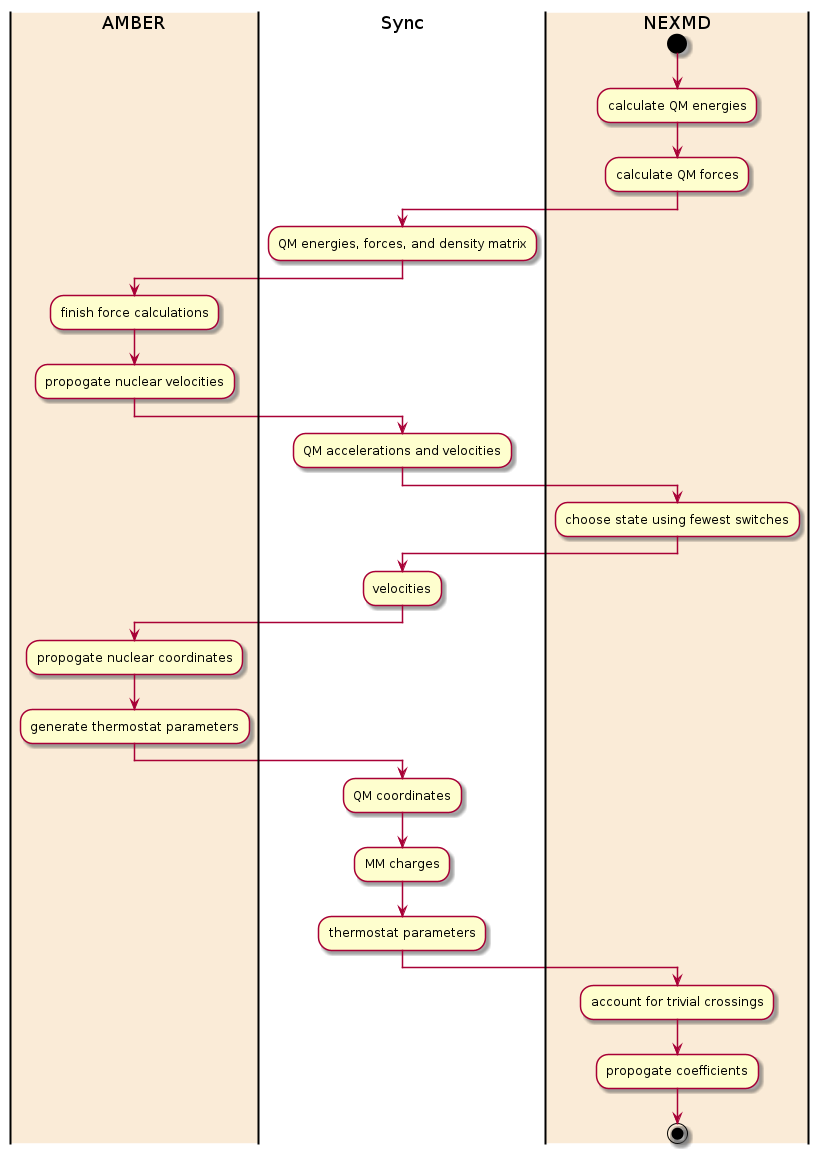
\includegraphics[width=0.7\linewidth]{../Paper2/scripted_diagrams/nasqm_overview.png}
  \captionof{figure}{Swim-lane diagram describing the common time-step of the SANDER-NEXMD interface.}
  \label{scheme:nasqm}
\end{minipage}\bigskip

The swim-lane chart in figure \ref{scheme:nasqm} describes a
common time-step that occurs within the SANDER-NEXMD
interface. With the coordinates provided by SANDER, NEXMD will
calculate and return to SANDER the energies and forces on the QM
atom and the excited-state density. With these results, SANDER
performs the final section of the QM/MM procedure as well as
determines the forces due to classical force fields to derive
the accelerations and velocities for the classical time-step. NEXMD then decides whether to perform a state transition
using the fewest switches algorithm, adjusting velocities as
needed to conserve energy. SANDER then propagates the nuclear
coordinates and generates a new set of random thermostat
parameters. NEXMD then checks if any trivial crossing occurs
within the potential energy surfaces. Once proper accounting
between the PESs and the energy order is determined, NEXMD
propagates the quantum coefficients.

When users initiate SANDER, they provide the usual SANDER inputs of coordinate,
parameter, and sander control files. An example of a SANDER ctrl file is shown in Figure
\ref{fig:ctrl}.

   \lstset{frame=single}
   \begin{mylisting}
     An example SANDER input file
     &ctrl
       ntx=5,
       ntb=1,
       ig=-1,
       taup=2.0,
       cut=16.0,
       tempi=300.0,
       temp0=300.0,
       ntt=3,
       gamma_ln=20.0,
       nstlim=2000,
       dt = 0.0005,
       ifqnt=1,
     /
     &qmmm
       scfconv=1.0E-8,
       qmmask=`:1',
       nae=1 ! Flag that links to NEXMD
     /
   \end{mylisting}
   \captionof{figure}{Example SANDER ctrl file for the SANDER-NEXMD interface}\label{fig:ctrl}
   \bigskip
   \setlength\parindent{24pt}
This file contains all the information regarding molecular dynamics, excluding most of the QM
calculations and all of the nonadiabtic parameters and is a standard input file to the AMBER
molecular dynamics programs.

To use NEXMD, the user will include the flag NAE under the QM/MM section of the input
file. This flag causes SANDER to call the NEXMD versions of the QM/MM force calculations instead of the default SQM routines. With the NEXMD force routine called, NEXMD will then look for the primary input file used in the stand-alone version of NEXMD, the input.ceon file. An example of this file is included below.

\lstset{frame=single}
\begin{mylisting}
&qmmm
    !***** Ground-State and Output Parameters
    qm_theory=`AM1', ! Integral type 
    verbosity=1, ! QM/MM output verbosity
    !***** Excited-State Parameters
    exst_method=1, ! CIS (1) or RPA (2) [1]
    dav_guess=1, ! Restart Davidson from (0) Scratch, (1) Previous,
    printcharges=1, ! (1) Print Mulliken Charges [0]
    !***** Solvent Models and External Electric Fields
    solvent_model=0, ! (0) None,
&endqmmm
&moldyn
    !***** General Parameters
    natoms=12, ! Number of atoms
    rnd_seed=19345, ! Seed for the random number generator bo_dynamics_flag=0, ! (0) Non-BO or (1) BO [1]
    exc_state_init=2, ! Initial excited-state (0 - ground state) [0]
    n_exc_states_propagate=3, ! Number of excited-states [0]
    !***** Dynamics Parameters
    n_quant_steps=4, ! Number of quantum steps for each classical step [4]
    num_deriv_step=1.0d-3, ! Displacement for numerical derivatives, A [1.0d-3]
    rk_tolerance=1.0d-7, ! Tolerance for the Runge-Kutta propagator [1.0d-7]
    !***** Non-Adiabatic Parameters
    decoher_type=2, ! (2) At successful plus frustrated hops...
    quant_step_reduction_factor=2.5d-2, ! Quantum step reduction factor [2.5d-2]
    !***** Thermostat Parameters
    therm_type=1, ! (1) Langevin | IGNORED,
    therm_temperature=300, ! Thermostat temperature, K | IGNORED
    therm_friction=20, ! Thermostat friction coefficient, 1/ps | IGNORED
    !***** Output & Log Parameters
    verbosity=3, ! NEXMD output verbosity (0-minimum, 3-maximum)
    out_data_steps=1, ! Number of steps to write data [1]
    out_coords_steps=10, ! Number of steps to write the restart file [10]
    out_data_cube=0, ! Write (1) or do not write (0) view files to generate cubes [0]
    out_count_init = 0, ! Initial count for view files [0]
&endmoldyn
&coord
    ! IGNORED
&endcoord
&veloc
    ! IGNORED
endveloc
&coeff
    0.00 0.00
    1.00 0.00
    0.00 0.00
&endcoeff
\end{mylisting}
%% \captionof{figure}{Example NEXMD input.ceon file for the SANDER-NEXMD interface}%\label{fig:inputceon}
\bigskip

Users can find additional flags and their corresponding options in the
NEXMD and AMBER documentation. The input.ceon file contains the
majority of the flags and preferences for the QM calculation and all
the non-adiabatic choices. The namespace QMMM exists in both the SANDER
ctrl file and the NEXMD input.ceon file. Both NEXMD and SANDER read
this namespace is into a shared struct due to NEXMD using SQM as a
backend; however, their respective parsers will look for different
flags. The SANDER parser will run first and will need the three flags
shown in \ref{fig:ctrl} to call the NEXMD routines. The NEXMD parser
for the QMMM namespace will then override anything else included in
both input files’ QM/MM namespace.

No modification to the input.ceon file is necessary from the stand-alone NEXMD code to run with SANDER. However, the coordinates
and velocities included in the file will be ignored, since SANDER
manages these data points. SANDER reads the coordinates and velocities
through the standard SANDER parameter and coordinates files
instead. Users can decide to leave these sections blank or to include
them, whatever their convenience. The preferences in the input.ceon file include the number
of QM steps between any classical time-step, the number of excited
states to include in the CIS calculation, the initial state, and the
initial coefficients. Note that a portion of this input file, such as
the thermostat preferences, relates to coordinate dynamics. SANDER
controls dynamics and will override these settings during
runtime. Users may want to remove these preferences from the
input.ceon file to avoid any confusion.

With the coordinates at time t = 0, NEXMD can calculate the energies in
a similar method described in Chapter 2. NEXMD is capable of
performing these energy calculations using Time-Dependent
Hartree-Fock, Time-Dependent Density Functional theory, or CIS. In
this work, we focus on the use of CIS. NEXMD can perform CIS
calculations using any of the semi-empirical methods available in SQM.
AM1 provides very reasonable computational cost to accuracy for our
systems of interest. It is the de-factor semi-empirical Hamiltonian
for organic conjugated molecules such as the one we will analyze in
chapters 4 and 5 \cite{silva2010benchmark} An analysis of parameter
choices can be found in previous
literature.\cite{nelson2012nonadiabatic} During the ground state
energy and density calculations, NEXMD heavily relies on slightly
modified SQM routines. These calculations follow the same principles
as described in the QM/MM section of Chapter 2. However,
unlike that section, we do not adequately account for the QM charges
during the QM-Ewald calculation. Proper treatment would require
multiple iterations of both the ground state SCF and the excited-state
Davidson algorithm. Further details of this problem as well as a
recommended solution can be found in the future works section of
Chapter 6. \cite{Walker2008} For a general time-step QM/MM interaction
will be added to the density matrix as follows:
\begin{enumerate}
\item Calculate the MM Ewald potentials using the classical charges
  from the MM atoms.
\item Construct the Hamiltonian matrix as if the QM region was in
  vacuum.
\item Add the one-electron terms for the interaction between QM
  atoms and the MM atoms within the cutoff to the Hamiltonian.
\item Within the SCF routine, copy the Hamiltonian to the Fock
  matrix and add the QM/MM two-electron integrals. When using AM1,
  SANDER expands the QM charge density into the STO-6G minimal
  basis set while treating the MM atoms as point charges, thereby
  providing the full electrostatic interaction between the QM and
  MM atoms.
\item Calculate the QM Ewald potential using the iteration’s
  Mulliken charges, then add the Ewald potentials for both QM and
  MM atoms to the Fock Matrix. Note that these Mulliken charges will be incorrectly from the ground state.
\item The SCF procedure continues until convergence resulting in a
  density matrix that incorporates solvents.
\end{enumerate}

NEXMD uses this ground-state density to perform a Davidson
diagonalization routine to determine the excited-state
energies. NEXMD then calculates the QM-QM forces using Equation
\ref{eq:NEXMDForces}. With the forces calculated, SANDER then
propagates the velocities by a single time-step. SANDER does not
yet adjust coordinates since NEXMD could still change these
velocities in the upcoming steps.

With the accelerations and velocities passed in by SANDER, NEXMD
then chooses to hop using the Tully fewest switches surface
hopping technique described in Chapter 2. If a hop occurs, NEXMD
adjusts the velocities in the non-adiabatic coupling vector’s
direction to conserve energy. If no hop occurs, then these
velocities remain unchanged.  Decoherence is then managed based
on user preferences. The current fully supported decoherence
methods are to either break coherence at any successful hop or to break at
any time where there is a high non-adiabatic coupling. Users may
also choose to ignore any decoherence correction.

We want to emphasize that at no point does SANDER know of the
multiple adiabatic states. SANDER simply propagates based on the forces and
velocities sent to it. SANDER then uses these new velocities to update
the atomic coordinates, which completes its time-step. SANDER then
begins a new time-step, generates a new set of thermostat parameters,
and forwards the new coordinates and parameters to NEXMD. NEXMD then
checks whether any trivial crossing occurred between the potential
energy surfaces by comparing the electron density matrices’ overlap.
\cite{nelson2012nonadiabatic} With the PESs correctly accounted for,
NEXMD then propagates the coefficients numerically using the
Runge-Kutta-Verner fifth-order and sixth-order method with the
coefficients described as
\begin{align}
  c_\alpha &= \sigma_\alpha e^{i\theta \alpha}\\
  \dot{\sigma}_\alpha &= - \sum_{\beta} \sigma_{\beta} \cos(\theta_{\beta} - \theta_{\alpha}) \dot{\mathbf{R}} \cdot \mathbf{d_{\alpha\beta}}\\
  -\hbar \sigma_\alpha \dot{\theta}_\alpha &= \sigma_\alpha \text{E}_\alpha + \hbar \sum_\beta \sigma_\beta \sin(\theta_{\beta} - \theta_\alpha)\dot{\mathbf{R}} \cdot \mathbf{d_{\alpha\beta}}.
\end{align}
NEXMD uses code developed by Hull, Enight, and Jackson to perform this calculation.\cite{hull1996runge}
Solvents are accounted for in the calculation of the Fock matrix during the ground-state SCF calculations. The non-adiabatic coupling terms are calculated numerically using Equation \ref{eq:NACouplingTerm}. The time derivative of the Fock matrix is determined using the differences of the elements between time-steps. This propagation does not require the calculation of intermediary forces.
Accurately calculating the non-adiabatic coupling terms requires a smaller time-step than what is necessary for nuclear coordinate propagation, and as such, we separate time-steps into smaller quantum time-steps. We use a procedure developed by Tully and Hammes-Schiffer to determine the chance of performing a hop over multiple time-steps.\cite{hammes1994proton}
In their work, they showed that
\begin{equation}
  g_{\alpha\beta} = \frac{\sum_j^{N_q} b_{\beta\alpha}(j) \delta t}{a_\alpha\alpha},
\end{equation}
where the number of intermidiary quantum steps per classical
propogation of the nuclear coordinates is described by \(N_q\). We
would need to calculate n(n-1) non-adiabatic coupling terms had we
allowed for more than a single hop to occur between time-steps. With
reasonable time-steps, the likelihood of more than a single hop
happening is extremely low; thus, we forbid the occurrence. This
restriction allows us to calculate only the non-adiabatic coupling from
the current excited-state.

In our work, we use four quantum time-steps for every classical time
step. Previous works demonstrate this as a reasonable number to use
for these parameters.\cite{nelson2012nonadiabatic} During each of
these quantum time-steps, NEXMD must calculate the energies and
non-adiabatic coupling terms. These calculations require interpolation
of the nuclear coordinates between the two classical time-steps. To
perform this interpolation, SANDER must pass the coordinates,
velocities, accelerations, and thermostat parameters to
NEXMD. However, this transfer is not very straightforward since NEXMD
uses a different time-step procedure than SANDER. For clarity, we will
first only look at the case of Newtonian mechanics without
excited-state transitions. When SANDER begins, it calculates a single
point calculation at time t = 0 and uses the calculated forces to
propagate the velocities (v) 1/2 a time-step (\(\delta\)) back. In its
main loop, it reperforms the energy and force calculation at time
t = 0. SANDER uses those accelerations to propagate v(t=-\(\delta\)/2) a
single time-step, making it the average velocity between t = 0 and
t=\(\delta\). It then moves the coordinates a time-step using this
average velocity. We show these coupled equations in equations
\ref{eq:SANDERNewtonian} and \ref{eq:SANDERNewtonian2}.

\begin{align}
  v(\delta/2) &= v(-\delta/2) + a(0)\delta \label{eq:SANDERNewtonian}\\
  x(\delta) &= x(0) + v(\delta/2) \delta \label{eq:SANDERNewtonian2}
\end{align}

NEXMD performs a theoretically equivalent algorithm but with numerical
differences. NEXMD calculates the energies and forces at t = 0 to move
the coordinates an entire time-step and the velocities a
half-time-step. It then calculates the acceleration for t = \(\delta\) using the
coordinates at t = \(\delta\) with which it uses to propagate the velocities the
last half of the time-step.
\begin{align}\label{eq:NEXMDNewtonian}
  x(\delta) &= x(0) + v(0)\delta + 1/2 a(0) \delta^2 \\
  v(\delta/2) &= v(0) + a(0)\delta/2\\
  v(\delta) &= v(\delta/2) + a(\delta)\delta/2
\end{align}
NEXMD does not calculate the energies and forces at time t = 0 twice as
performed in SANDER. The SCF calculation uses the previously
calculated density matrix for its initial guess. Because SANDER will
perform, at minimum, two iterations during an SCF calculation, the
forces and energies produced by NEXMD for the first step will differ
slightly from those produced by SANDER even though they use the same
SCF routines. These small differences between the two programs in the
first step will lead to larger differences later. However, both
programs still return qualitatively identical results.

SANDER never calculates the velocities between time-steps.  As such,
the half-step velocities needed by NEXMD for the calculations of the
non-adiabatic coupling vectors and the interpolation of the QM steps
need to be the average of the old and new velocities in SANDER.

Using the Langevin thermostat, NEXMD will also require the generated
random variables for the thermostat generated by AMBER to determine
the stochastic forces used in the QM
interpolation.\cite{paterlini1998constant} In AMBER, the Langevin
thermostat is accounted for in the coordinate propogation
\begin{align}
  x(\delta) &= x(0) + v(\delta/2) t\\
  x(\delta) &= x(0) + \left(v(-\delta/2) c_e + (F(0) + R(0)) \frac{c_i \delta}{m} \right) \delta,
\end{align}
where \(F(0)\) is the force at t = 0, m the mass of the atom, and
\(R(0)\) a random perturbation generated by a gaussian distribution
dependent on the temperature, atom mass, time-step and friction
coefficient.  The coefficients \(c_e\) and \(c_i\) are based of the
Langevin friction coefficient \(\gamma\)
\begin{align}
  c_e &= 1 - \frac{\gamma\delta}{2}\\
  c_e &= \frac{1}{1 + \frac{\gamma \delta}{2}}.
\end{align}
In NEXMD, the Langevin equations are also included in the coordinate propogation but as
\begin{align}
  x(\delta) = x(0) + (v'(0)\chi_v + a'(0)\chi_a + P_r),
\end{align}
where \(\chi_v\), \(\chi_a\), and \(P_r\) are the fricition, intertia,
and stochastic forces repectively.  The prime indicates the variable
is in atomic units as opposed to the units used in SANDER.

This can be expanded to 
\begin{align}
  x(\delta) = x(0) + ((v'(-\frac{\delta}{2}) + \frac{1}{2}a'(0)\chi_v + V_r(-\delta))\chi_v + a'(0)\chi_a + P_r),
\end{align}
where \(V_r\) is a random perturbation to the velocities.
\(\chi_v\) and \(\chi_a\) are non-random variables and can be generated by NEXMD by feeding NEXMD the Langevin friction coefficient \(\gamma\).
With a bit of algebra, the convertion from SANDER to NEXMD for the random variable can be derived to be
\begin{align}
  V_r &= \frac{1}{2}(v(\delta/2) - v(-\delta/2))\nu_{an} - \frac{1}{2}a'(0)\chi_v\\
  P_r &= v(\delta/2)) - \left( \frac{1}{2} (v(-\delta/2) + v(\delta/2))\nu_{an}\chi_v + a'(0)\chi_a \right),
\end{align}
where \(\nu_{an} \approx 9.35E-4\) is a unit convertion from SANDER to NEXMD.

Once the quantum coefficients are propogated, the cycle continues with
the calculations of the QM/MM energies.

\section{Benchmarks}
    \noindent
    \begin{multiFigure} 
      \addFigure{0.45}{./Images/Timings/bo_npropogated}
      \addFigure{0.45}{./Images/Timings/bo_nsolvents}
      \captionof{figure}[Adiabatic timings]{Run time per time-step for PPV\(_3\)-NO\(_2\) with 3254 explicit methanol solvents during adiabatic dynamics.}
      \label{fig:adiabaticTimings}
    \end{multiFigure}\bigskip

    \noindent
    \begin{multiFigure} 
      \addFigure{0.45}{./Images/Timings/nbo_npropogated}
      \addFigure{0.45}{./Images/Timings/nbo_nsolvents}
      \captionof{figure}[Non-adiabatic timings]{Run time per time-step for PPV\(_3\)-NO\(_2\) with 3254 explicit methanol solvents during non-adiabatic dynamics.}
      \label{fig:nonadiabaticTimings}
    \end{multiFigure}\bigskip



Figures \ref{fig:adiabaticTimings} and \ref{fig:nonadiabaticTimings} show the timings for the Sander-NEXMD interfaces. 
Benchmarks consisted of a single PPV\(_3\)-NO\(_2\) molecule surrounded by 3254 CH\(_3\)OH molecules.
PPV\(_3\)-NO\(_2\) consists of 50 atoms, and every additional CH\(_3\)OH molecule adds 6 atoms for 19,754 atoms total.
We vary both the number of solvents included in the QM region and the number of excited-states propagated.
We performed these calculations on an AMD Ryzen 5 3600XT. Results are averaged over 8 trajectories. The initial coordinates and velocities for these 8 trajectories were sampled from a 320 ps ground state MM trajectory. Each datapoint shares these same initial conditions. Each trajectory ran for 30 0.5 fs time-steps, and the results are averaged over time.

Non-adiabatic trajectories requires roughly an order of magnitude more computational time than the corresponding adiabatic cases. Increasing the number of states increases the computational costs nearly linearly, as expected for configuration interaction calculations. The computational costs for adding solvents into the QM region increase superlinearly, expected while using semi-empirical methods. Therefore, we are limited in the number of solvents we can include in the QM region and will need to be selective in which we choose.

Results for ground-state QM/MM dynamics using the SANDER-NEXMD interface were identical to those with SANDER using the default SQM library with and without using a thermostat. This is due to NEXMD using this same SQM library for a backend. Results from the interface for non-adiabatic dynamics in vacuum are nearly identical to those produced from NEXMD alone. A minor difference occurs due to SANDER performing the initial energy and force calculations twice while NEXMD only performs it once. For single-point calculations, these results are identical.
% Modified from old template.
\chapter{Spectroscopic Analysis of PPV\(_3\)-NO\(_2\)}

\section{Introduction}
NEXMD is an efficient program for the simulation of photoinduced
dynamics of extended conjugated molecular systems involving manifolds
of coupled electronic excited states over timescales extending up to
tens of picoseconds. \cite{sifain2018photoexcited, Bjorgaard2015,
  case2020a, tretiak02_densit_matrix_analy_simul_elect,
  malone2020nexmd} It includes solvent effects using implicit
models. These implicit solvents provide insight into the electrostatic
forces. Still, explicit solvents should provide additional information
about the quantum or steric effects, allowing the simulation of
electron transfer processes due to the stabilization of charge
separation in the excited state.\cite{woo2005solvent}  Many multichromophoric molecular
systems are soluble in polar solvents such as water. Such simulations
could provide sought-after insight into the effects of charged side
groups on the structural sampling, structural rearrangement, and
transition density redistribution during electronic relaxation.

Adequate sampling of the solvent and solute configuration space,
including hundreds to thousands of solvent molecules, currently
cannot be achieved by QM calculations alone due to the \hlc{large}
computational cost of such extensive
systems. \cite{barbatti2011nonadiabatic} QM/MM methods exist to allow
the computationally expensive QM calculations to be performed only on
the area of interest while propagating the rest of the system with
cheaper classical dynamics.  The SANDER program in the AMBER
molecular dynamics package performs classical molecular dynamics
using periodic boundary conditions with high optimization.  SANDER
with QM/MM performs well with tens of thousands of MM atoms and
currently calculates QM/MM with semi-empirical Hamiltonians and DFT;
however, previous versions did not provide options for excited-state
MD.

In this work, we redirect AMBER's SANDER package from its usual
semi-empirical QM package, SQM, to a modified NEXMD library.
SANDER linked to the NEXMD library performs adiabatic dynamics at
ground-state and CIS excited-state potential energy surfaces on
~100 atoms at QM and 1000s at MM.  We apply our method to an
analysis of a three-ring para-phenylene vinylene oligomer
\((PPV_{3}-NO_{2})\).  We look at how explicit solvents affect \(PPV_{3}-NO_{2}\)'s
absorption and emission spectra as well as its geometric structure.

\section{Simulation Methods}

\noindent
\begin{minipage}[c]{\textwidth}
  \centering
  \includegraphics[width=5in]{../Paper1/Images/trajectory_diagram/trajectories.pdf}
  \captionof{figure}{Description of the adiabatic simulation}
  \label{fig:adiabaticDynamics}
\end{minipage}\bigskip

Figure \ref{fig:adiabaticDynamics} visually describes the layout of our simulations performed in vacuum, methanol, chloroform, and carbon tetrachloride.
   First, we performed a 320 ps molecular dynamics simulation at the ground state (S0) at 300K (NVT) using the General AMBER Force Field and periodic boundary conditions, as guided from previous convergence studies. \cite{silva2010benchmark}
We set the classical time-step to 0.5 fs and use a Langevin thermostat with friction constant 2 ps\(^{-1}\) throughout all simulations. The choices for these parameters were based on work aimed at optimizing these choices in NEXMD. \cite{nelson2012nonadiabatic}
   128 evenly-spaced snapshots were then collected from the MM simulation and used as initial conditions for 128 individual 10 ps simulations using the semi-empirical AM1 QM/MM ground state Hamiltonian that has been shown to provide reasonable accuracy for the computational cost. \cite{silva2010benchmark} We use the data collected from these trajectories for the absorption calculation.
   The resulting geometries of these ground-state QM/MM simulations were then used as the initial geometrical configuration of a final excited-state simulation. Each configuration was vertically excited to the lowest excited state with no regard to coupling or energy conservation. We propagate these excited-state QM trajectories using configuration interaction singles (CIS) with the AM1 Hamiltonian, 
   The CIS calculations include the first 9 excited states of the PPV\(_3\)-NO\(_2\) molecule and \hlc{up to 20} solvent molecules closest to the central phenyl.
   We treat all other solvent molecules using classical dynamics.
   We restrict the QM solvents from drifting away from the solute and the other MM solvents from drifting closer than these QM solvents.

\noindent
	  \begin{multiFigure} 
	    \addFigure{0.45}{../Paper1/Images/ppvno2.png}
	    \addFigure{0.45}{../Paper1/Images/vacuum-td.png}
	    \captionof{figure}{A) Diagram of PPV\(_3\)-NO\(_2\) showing the bonds of interest. B) Transition density from ground to excited state.}
	    \label{fig:PPV3NO2}
	  \end{multiFigure}
\bigskip

As shown in Figure \ref{fig:PPV3NO2} B, the S0-S1 transition density resides towards the center of the molecule on the vinyl groups nearest to the central phenyl group.
Charge movements on solvents far from this concentration of density should cause negligible effects on transition characteristics.
To maximize the QM/MM calculation utility, we only include the solute and the solvent molecules nearest to this central phenyl group in the QM calculations.
To prevent these solvents from drifting during the trajectories, we implement a simple harmonic restraint using AMBER's NMR restraints with a force constant of 200 KCal/mol \AA\(^{-2}\).
We select the N solvent molecules based on the minimum atom-atom distance between the solvent and the central phenyl group.
We then restrain these solvents using the harmonic constraint on the distance from the center of geometry of the solvent to the center of geometry of the central phenyl group.
We also use the same restraint to prevent the solvent molecules not included in the QM calculation from getting closer to the central phenyl than the QM solvents, effectively making a spherical shield around the solute's central phenyl group.
Since the distance between the center of geometries and the closest atoms are not necessarily equal, solvent atoms could initially be pushed either inside or outside this shield during the transition from MM to QM.
However, this push only occurs during the initial equilibration of the QM ground-state calculations excluded from any analysis.
Once the QM calculations begin, these constraints persist throughout all further calculations.
The average radii for the restraint barriers are shown Table \ref{tab:restraints}.

\begin{table}[H]
  \caption[Restraint radii]{The radius in \AA\ of the restraint shield averaged over trajectories for varying number of solvents included in the QM region.} \label{tab:restraints}
  % \begin{center}
  \begin{tabularx}{\textwidth}{XXXXXXXXX}\hline
    Solvent   & 5  & 10 & 20 \\\hline
    CCl\(_4\)  & 6.3  & 7.5    & 9.7 \\
    CH\(_3\)OH & 5.5 &  6.5   & 8.0 \\
    CHCl\(_3\) & 6.3 &  7.6   & 9.4 \\\hline
  \end{tabularx}
\end{table}

\section{Results}

\subsection{Spectra}

Energies, coordinates, and dipole information are acquired every ten steps.
Equilibration times from either MM to QM state or from S0 to S1 range from 2-4 ps.
As such, we exclude the first four ps of each trajectory in calculating the spectra in data analysis for the absorption and emission analysis. 

The solvent's polarizability should affect the transition dipole moments and thus the corresponding spectra.  This effect has been shown experimentally. \cite{marcus1956electrostatic,martin1998hydrolysis,Park2013,LeDroumaguet2005}.
Such shifts are referred to as solvatochromic shifts.
Previous studies have analyzed solvatochromic shifts in conjugated substituted PPV\(_3\)-NO\(_2\) molecules with the NEXMD program in implicit solvents.\cite{Santhanamoorthi2009}
Results with NEXMD by TD-AM1 were redshifted from the experimental results, while single-point calculations using TD-CAM-B3LYP provided by G09 in the same implicit solvent were blue shifted.
Other NEXMD computations have shown comparable redshifts in spectra of similar molecules in implicit solvents compared to experiment. \cite{Bjorgaard2015}
We performed similar calculations in this paper; however, in explicit solvent.
We compare the results to those presented in implicit solvent.

We collect the vertical excitation dipoles and oscillator strengths between the ground state S0 and S1 every five fs during each trajectory's steady-state to produce the absorption/emission spectra of PPV\(_3\)-NO\(_2\).
We sum over excitation states averaged over the geometries and broaden the spectra using a Gaussian bin function with FWHM=0.16 eV corresponding to a 100 fs FWHM laser excitation.
We normalized it such that the maximum absorption is 1. 

\noindent
\begin{multiFigure} 
  \addFigure{0.45}{../Paper1/Images/spectra_abs_compared.png}
  \addFigure{0.45}{../Paper1/Images/spectra_flu_compared.png}
  \captionof{figure}[Fluorescence and absorption spectra in various solvents]{PPV\(_3\)-NO\(_2\) A) absorption and B) fluorescence spectra in various solvents with 20 included in QM region.}
  \label{fig:spectrasolvents}
\end{multiFigure}\bigskip

\noindent
\begin{multiFigure} 
  \addFigure{0.45}{../Paper1/Images/nquant_abs_comparison.png}
  \addFigure{0.45}{../Paper1/Images/nquant_flu_comparison.png}
  \captionof{figure}[Fluorescence and absorption spectra by number of quantum solvents]{PPV\(_3\)-NO\(_2\) A) absorption and B) fluorescence spectra in CCL\(_4\) with varying number of QM solvents.}
  \label{fig:spectranquant}
\end{multiFigure}\bigskip

Figure \ref{fig:spectrasolvents} A presents the absorption spectra for PPV\(_3\)-NO\(_2\) in select solvents and vacuum.
The shown absorption has contributions from the nine lowest energy excited states, though the S1 state is the primary contributor to the spectra.
We found the number of solvent molecules included in the QM region caused only minor deviations in the spectra, with the largest variance (0.02~eV) occurring between the 20QM and MM carbon tetrachloride systems, as seen in Figure \ref{fig:spectrasolvents}. As such, we only present results from trajectories with 20 QM solvents.
The broad absorption and fluorescence bands are common features of conjugated materials due to the large geometric relaxation in the lowest excited state. \cite{bredas2009molecular}
All solvent results are redshifted from those in vacuum matching findings in previous works.\cite{Park2013}
In Figure \ref{fig:spectranquant}, the absorbance within methanol and chloroform were very similar, with a peak shift from vacuum of -0.04 eV.
Within carbon tetrachloride, the magnitude of this shift increases slightly more to-0.06 eV. 

Aligning with previously reported results, the fluorescence calculations found in Figure \ref{fig:spectranquant} show an overall more intense redshift from vacuum, along with a more significant dispersion among the solvents. \cite{Park2013}
The smallest shift, at -0.06 eV, occurs in carbon tetrachloride, while the largest, at -0.12 eV, occurs in methanol.
Previous works have demonstrated that the energy levels of PPV\(_3\)-NO\(_2\) are further stabilized by more polar solvents, a feature clearly seen by our results.\cite{Park2013,woo2005solvent}

\subsection{Potential Energy Relaxation}

\noindent
\begin{minipage}[c]{\textwidth}
  \centering
  \includegraphics[width=5in]{../Paper1/Images/energies.png}
  \captionof{figure}[Potential energy relaxation during adiabatic dynamics]{Potential energ for states S0 and S1 for PPV\(_3\)NO\(_2\) with 20 solvent molecules included in the QM region as the system relaxes on the S1 PES. Energies are reported as differences from the ground state at t = 0.}
  \label{fig:energiesAdiabatic}
\end{minipage}\bigskip

The peaks of absorption and the fluorescence properties should correspond strongly with the difference between the ground state (S0) and the first excited state (S1) energies at the point of transistion.
Figure \ref{fig:energiesAdiabatic} shows the energies for states S0 and S1 averaged over 128 trajectories for PPV\(_3\)-NO\(_2\) in the various solvents with 20 solvent molecules included in the QM calculations.
During the first four ps in the chart, the system runs on the ground-state S0, and the S0 energies stay near the minimum with small oscillations caused by temperature.
At time t = 0, the system instantaneously hops to the S1 potential energy surface.
The average energy difference of around 2.95 eV at t = 0 corresponds reasonably well with whats seen in the absorption spectrums' peaks where little difference is seen between the solvents. During the first 10-20 fs of this calculation, the ground state energy rapidly increases, suggesting an ultra-fast geometric relaxation process occurs. The molecule then seems to experiences a slower, ~2 ps, relaxation process.
As expected the final energy values at t = 10 ps for S0 and S1 are higher and lower, respectively, than they were when t < 0.
Unexpectedly, PPV\(_3\)-NO\(_2\) in methanol seems to experience a minimum in s1 energy at around t = 2 ps then steadily increase until around t = 8 ps. During this time, the S0 energy also increases, alowing the energy difference found in methanol to remain lower than that found in other solvents which aligns well with the red shift found in the fluorescence calculations. This may be due to solvent rearrangement, however further inspection did not lead to anything conclusive.

\subsection{Bond Length Alternation}
    In \(\pi\) conjugated organic compounds, the electrons unevenly distribute across the carbon-carbon \(\pi\) bonds, causing a dimerization or alternation of single-like carbon bonds and double-like carbon bonds.
    When promoted from the highest occupied molecular orbital (HOMO) to the lowest occupied molecular orbital (LOMO), the bonding-antibonding pattern switches, and the electron densities correspondingly adjust.
    As a result, the single-like carbons become more double-like and vice versa. \cite{bredas1999excited}
    This structural difference between the excited-state and ground-state of PPV3-molecules is presented clearly by distortions in the C=C and C-C bonds found in the vinylene segment.\cite{tretiak02_densit_matrix_analy_simul_elect, karabunarliev2000rigorous, karabunarliev2000adiabatic, nelson2014nonadiabatic}
    These distortions can be measure by bond length alternation (BLA)
    \begin{equation}
      \frac{d_i + d_e}{2} - d_c,
    \end{equation}
    where \(d_i\) and \(d_e\) are the interior and exterior bonds, and \(d_c\) is the central bond.
    This value represents the differences between the double and single bonds of the vinylene sections.
    The BLA is a descriptor for \(\pi\) bond distributions. \cite{tretiak2002conformational}
    For this system, we analyze the BLAs of two separate bond sets, the bonds d1-3 (near-set) and d4-6 (far-set) seen in Figure \ref{fig:PPV3NO2} A. 

    \noindent
    \begin{minipage}[c]{\textwidth} 
      \centering
      \includegraphics[width=6in]{../Paper1/Images/bla.png}
      \captionof{figure}[BLA of bonds during adiabatic dynamics]{BLA of bonds d1-3 (left) and d4-6 (right) during the last 4 ps of the S0 dynamics and 10 ps of the S1 dynamics.
        QM energy and force calculations include the 20 solvents nearest the central ring.}
      \label{fig:bla_adiabatic}
    \end{minipage}\bigskip


    \begin{table}[H]
      \caption[Adiabatic bond length alternation]{Bond Length Alternation (BLA) summary for PPV\(_3\)-NO\(_2\) in various solvents with 20 solvents included in the QM region.} \label{tab:adiabaticBLA}
      % \begin{center}
      \begin{tabularx}{\textwidth}{XXXXXXXXX}\hline
        Molecule   & d\(_1\)  & d\(_2\) & d\(_3\) & BLA\(_{\textbf{near}}\) & d\(_1\)  & d\(_2\) & d\(_3\) & BLA\(_{\textbf{far}}\)\\\hline
        Vacuum     & 1.429     & 1.375    & 1.418    & 0.049              & 1.441     & 1.365    & 1.427   & 0.069\\
        CCl\(_4\)  & 1.427     & 1.376    & 1.417    & 0.046              & 1.441     & 1.365    & 1.426   & 0.068\\
        CH\(_3\)OH & 1.422     & 1.382    & 1.415    & 0.037              & 1.444     & 1.362    & 1.431   & 0.076\\
        CHCl\(_3\) & 1.423     & 1.380    & 1.415    & 0.039              & 1.443     & 1.365    & 1.429   & 0.074\\\hline
      \end{tabularx}
    \end{table}

    Figure \ref{fig:bla_adiabatic} shows the bond length alternation of
    PPV\(_3\)-NO\(_2\) in various solvents during the last 4 ps of the S0 trajectories and the 10 ps of the S1 trajectories. At time t = 0, the systems instantaneously transition from S0 to S1.
    Within the first couple hundred femtoseconds after the
    excitation to S1, the central bonds (d2 and d5) expand, while the interior (d3 and d6) and
    exterior bonds (d1 and d4)  contract.  This bond restructuring is amplified by
    proximity to the nitro group for all solvent environments, where we
    see an average drop of 0.07 Å in sets d1-3 compared to a 0.04 Å drop
    found in sets d4-6.  This amplification's strength depends on the
    solvent environment where the BLA difference between the far and near
    sets PPV\(_3\)-NO\(_2\) in methanol, 0.034 Å, surpasses that found in carbon
    tetrachloride, 0.022 Å.

    Table \ref{tab:adiabaticBLA} presents further details of the S1 BLA simulation.
    The information presented is averaged over time after relaxation across all trajectories.
    In all cases, the exterior bonds become slightly longer than the interior bond.
    The BLAs from the near and far sets split.
    In the near set, the S0 and S1 BLA converge to 0.1091 Å and 0.00453 Å, respectively.
    In the far set, these numbers are 0.1103 Å and 0.0697 Å, respectively.
    The smaller bond length spread in the near set and the lower BLA suggest more delocalization on those bonds than in the far set. 
    The number of solvents included in the QM calculations had little effect on the convergence of the distances or BLA.
    PPV\(_3\)-NO\(_2\) had similar ground state BLAs of around 0.11 Å for both near and far sets matching results on similar systems regardless of the solvent. \cite{nelson2011nonadiabatic}
    The S1 BLAs varied between the solvents and the distance away from the nitro group.
    PPV\(_3\)-NO\(_2\) presents the smallest near set S1 BLA and largest far set S1 BLA when in methanol in comparison to the other tested solvents.
In carbon tetracholoride, it shows similar behavior to vacuum, presenting the largest near set S1 BLA and the smallest far set S1 BLA out of the solvents tested.

\subsection{Wiberg Bond Orders}
\begin{minipage}[c]{\textwidth}
  \centering
  \includegraphics[width=5in]{../Paper1/Images/ccl4-5s-widberg.png}
  \captionof{figure}[Wiberg Bond Orders During Adiabatic Dynamics.]{Wiberg Bond Orders for PPV\(_3\)-NO\(_2\) in CCL\(_4\) with 5QM Solvents During Adiabatic Dynamics. }
  \label{fig:bondOrdersAdiabatic}
\end{minipage}\bigskip

The significant effects of the S0-S1 transitions on the Cartesian measurement of BLA encourages the analysis of these bonds' quantum mechanical behavior.
Because the double-bonds elongate and the single-bonds contract, we expect the single-bonds to gain a partial double-bond character and vice versa.
Simple bond ordering does not consider these subtleties of a quantum electronic wave-function.
Fortunately, the quantum mechanical descriptor, the Wiberg bond index, provides a reasonable analogy of the classical Lewis structure a chemist would expect.
Wiberg bond indexes are calculated from the density matrix by 
\begin{equation}
  W_{AB} = \sum_{\mu\in A}\sum_{\nu \in B} | D_{\mu\nu} |^2,
\end{equation}
where \(A\) and \(B\) are indexes of the two atoms, \(\mu\) and \(\nu\) are the atomic orbitals, and \(D\) is the density matrix.
The method sums the electron density shared by both atoms.
If an electron is fully localized on a single atom, the sum of the elements equals zero providing a value that matches our intuition. 

As the bond order increases, we expect the bond to become more rigid and the bond length to shrink.
Figure \ref{fig:bondOrdersAdiabatic} displays the bond order of bonds d1-6 for PPV\(_3\)-NO\(_2\) in carbon tetrachloride with 5 QM solvent molecules included in the QM region.
At time t = 0, the system instantaneously transitions to the first excited state, S1.
The Wiberg bond index then uses the density matrix for S1, leading to a sudden shift in its value.
At S1, the bond orders of d2 and d5 instantaneously drop, and expansion of their bond lengths soon follows.
The larger shifts in the near set correspond to the information found in the BLA analysis.
The interior bonds (d1 and d4) have lower bond indexes than their exterior counterparts (d3 and d6).

\subsection{Torsional Angles}

\noindent
\begin{minipage}[c]{\textwidth}
  \centering
  \includegraphics[width=6in]{../Paper1/Images/dihedrals.png}
  \captionof{figure}[Torsional angles during adiabatic dynamics]{Torsional angle around d1-d3, near, and d4-d6, far, in S1 within various solvents with 20 solvents included in the QM region.}
  \label{fig:dihedralAdiabatic}
\end{minipage}\bigskip

\begin{table}[H]
  \caption{Adiabatic excited state torsional angle Relaxation} \label{tab:adiabaticDihedrals}
  % \begin{center}
  \begin{tabularx}{\textwidth}{XXXXX}\hline
    Molecule    & S0 Near  & S1 Near & S0 Far & S1 Far\\\hline
    Vacuum      & 28.0 \(\pm\) 1.0\(^\circ\) & 12.5 \(\pm\) 0.5\(^\circ\) & 28.5 \(\pm\) 0.9\(^\circ\) & 17.4 \(\pm\) 0.8\(^\circ\)\\
    CCl\(_4\)  & 25.7 \(\pm\) 0.8\(^\circ\)  & 12.5 \(\pm\) 0.6\(^\circ\) & 24.5 \(\pm\) 1.1\(^\circ\) & 14.5 \(\pm\) 0.6\(^\circ\)\\
    CH\(_3\)OH  & 26.4 \(\pm\) 1.0\(^\circ\)  & 11.7 \(\pm\) 0.7\(^\circ\) & 28.1 \(\pm\) 0.9\(^\circ\) & 16.1 \(\pm\) 0.6\(^\circ\)\\
    CHCl\(_3\)  & 25.1 \(\pm\) 0.9\(^\circ\)  & 11.8 \(\pm\) 0.5\(^\circ\) & 26.2 \(\pm\) 1.0\(^\circ\) & 15.7 \(\pm\) 0.6\(^\circ\)\\\hline
  \end{tabularx}
\end{table}

As we've seen, in the ground, A\(_g\) state, the \(\pi\) bonds along the vinylene segments experience significant electronic spin alternation. Immediately after excitation, PPV\(_3\)-NO\(_2\) transitions from this A\(_g\) state to the lowest excited state that possesses B\(_u\) symmetry, which allows the dispersion of the electrons across these segment and a reduction in this alternation. As the single-bonds gain more double-bond-like characteristics, the segment begins to encourage a more planar configuration.  The torsion angle around the vinylene segments is highly coupled to the excited state.\cite{nelson2011nonadiabatic,panda2013electronically}
We can, therefore, following precedent, use the torsion angle around the vinylene segments as the slow nuclear coordinates of PPV\(_3\)-NO\(_2\). \cite{Clark2012,barford2011ultrafast}
Torsion angles around d1 and d3 (near) and d4 and d6 (far) are averaged over 128 trajectories to produce the torsion angles data shown in Figure \ref{fig:dihedralAdiabatic} and Table \ref{tab:adiabaticDihedrals}.

Figure \ref{fig:dihedralAdiabatic} shows these torsional angles for PPV\(_3\)-NO\(_2\) within our test solvents. Once again, at time t = 0, the molecule is excite from S0 to S1.  
Table \ref{tab:adiabaticDihedrals} shows a summary of the torsion angles analysis of all tested solvents after five ps of relaxation after the jump to the first excited state.
The trajectories include 20 solvent molecules within the QM calculations.
A noticeable shift towards a planar geometry occurs in all solvents.
This shift is greatest near the nitro group.
% Modified from old template.
\chapter{QM/MM Non-adiabatic Dynamics of PPV\(_3\)-NO\(_2\)}

\section{Introduction}

\section{Simulation Methods}

\noindent
\begin{minipage}[c]{\textwidth}
  \centering
  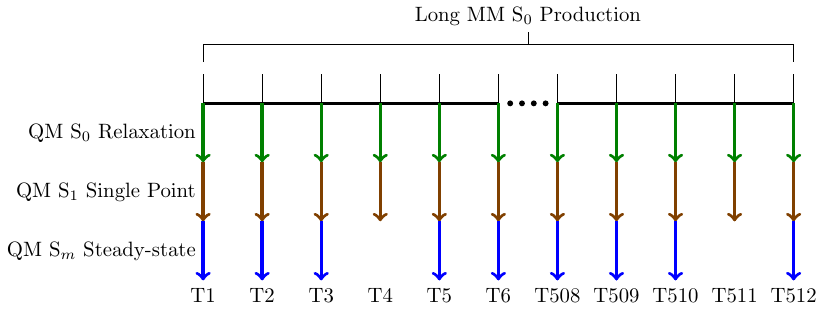
\includegraphics[width=5in]{../Paper2/scripted_diagrams/simulations-1.png}
  \captionof{figure}{Diagram of the Nonadiabatic dyanmics simulation.}
  \label{fig:nonadiabaticSimulation}
\end{minipage}\bigskip

We equilibrated the system to a temperature set to 300K. To collect a broad
enough sampling, we sampled from a 1024 ps, with a 0.5 fs timestep fully
classical trajectories using the AMBER force field. We performed a separate
trajectory for each situation combination of solute / with solvent including
whether the solvent was included in the QM calculations. We had a total of 6
separate 1024 ps classical trajectories, PPV3 in Vacuum, CH\(_3\)OH, and 5QM CH\(_3\)OH
and PPV\(_3\)-NO\(_2\) in Vacuum, CH\(_3\)OH, and 5QM CH\(_3\)OH. 1024 snapshots where taken at
1ps, 2ps .. 1024ps. We used the final frame of those tranjectories as the
initial conditions for an additional 4ps using the AM1 semiempical Hamiltonian
Born-Oppenheimer on the molecules to be included in future QM calculations to
allow the system to relax. The 4 ps timescale was determined using the
information form the previous paper. The simulations were described the Langevin
equations at a temperature set to 300 K with the Langevin friction parameter set
to 2 ps\(^{-1}\). The final frames of these QM trajectories were then used as the
initial conditions for the following pulse pump calculations.

Pump-Probe Spectroscopy is an experimental technique commonly performed in the
study of ultrafast electonic statte dynamics. In the case of conjugated polymers
in can be used to study the localized excictronic transitions that are
accessible through an excitation from the S1 state but not the ground state S0.
To simulate this behavior, we take the final snapshot of the QM ground state
calculations and perform a single point calculation at the S1 state to find the
next state with the highest oscillator strength.

The unnormalized probabilities are determined using
    \begin{equation}
      P'(\Omega_e) = f_{ge}(\Omega_e) \times \frac{1}{\sqrt{2\pi \sigma^2}} \exp \left[ - \frac{(\Omega_e - \Omega)^2}{2\sigma^2} \right]
    \end{equation}
where \(\Omega\) is the energy of the laser exciatation, \(\Omega_\alpha\) the energy difference from the ground state at excited state \(\alpha\), \(f_{ge}(\Omega_e)\) is oscillator strength, and \(\sigma\) the spectral broadening.  

The probability of initially populating an excited state \(\alpha\) is then
\begin{equation}
  P(\Omega_\alpha) = \frac{P'(\Omega_i)}{\sum_i P'(\Omega_i)}
\end{equation}

\section{Results}

\subsection{Intitial Excitations}

\noindent
\begin{minipage}[c]{\textwidth}
  \centering
  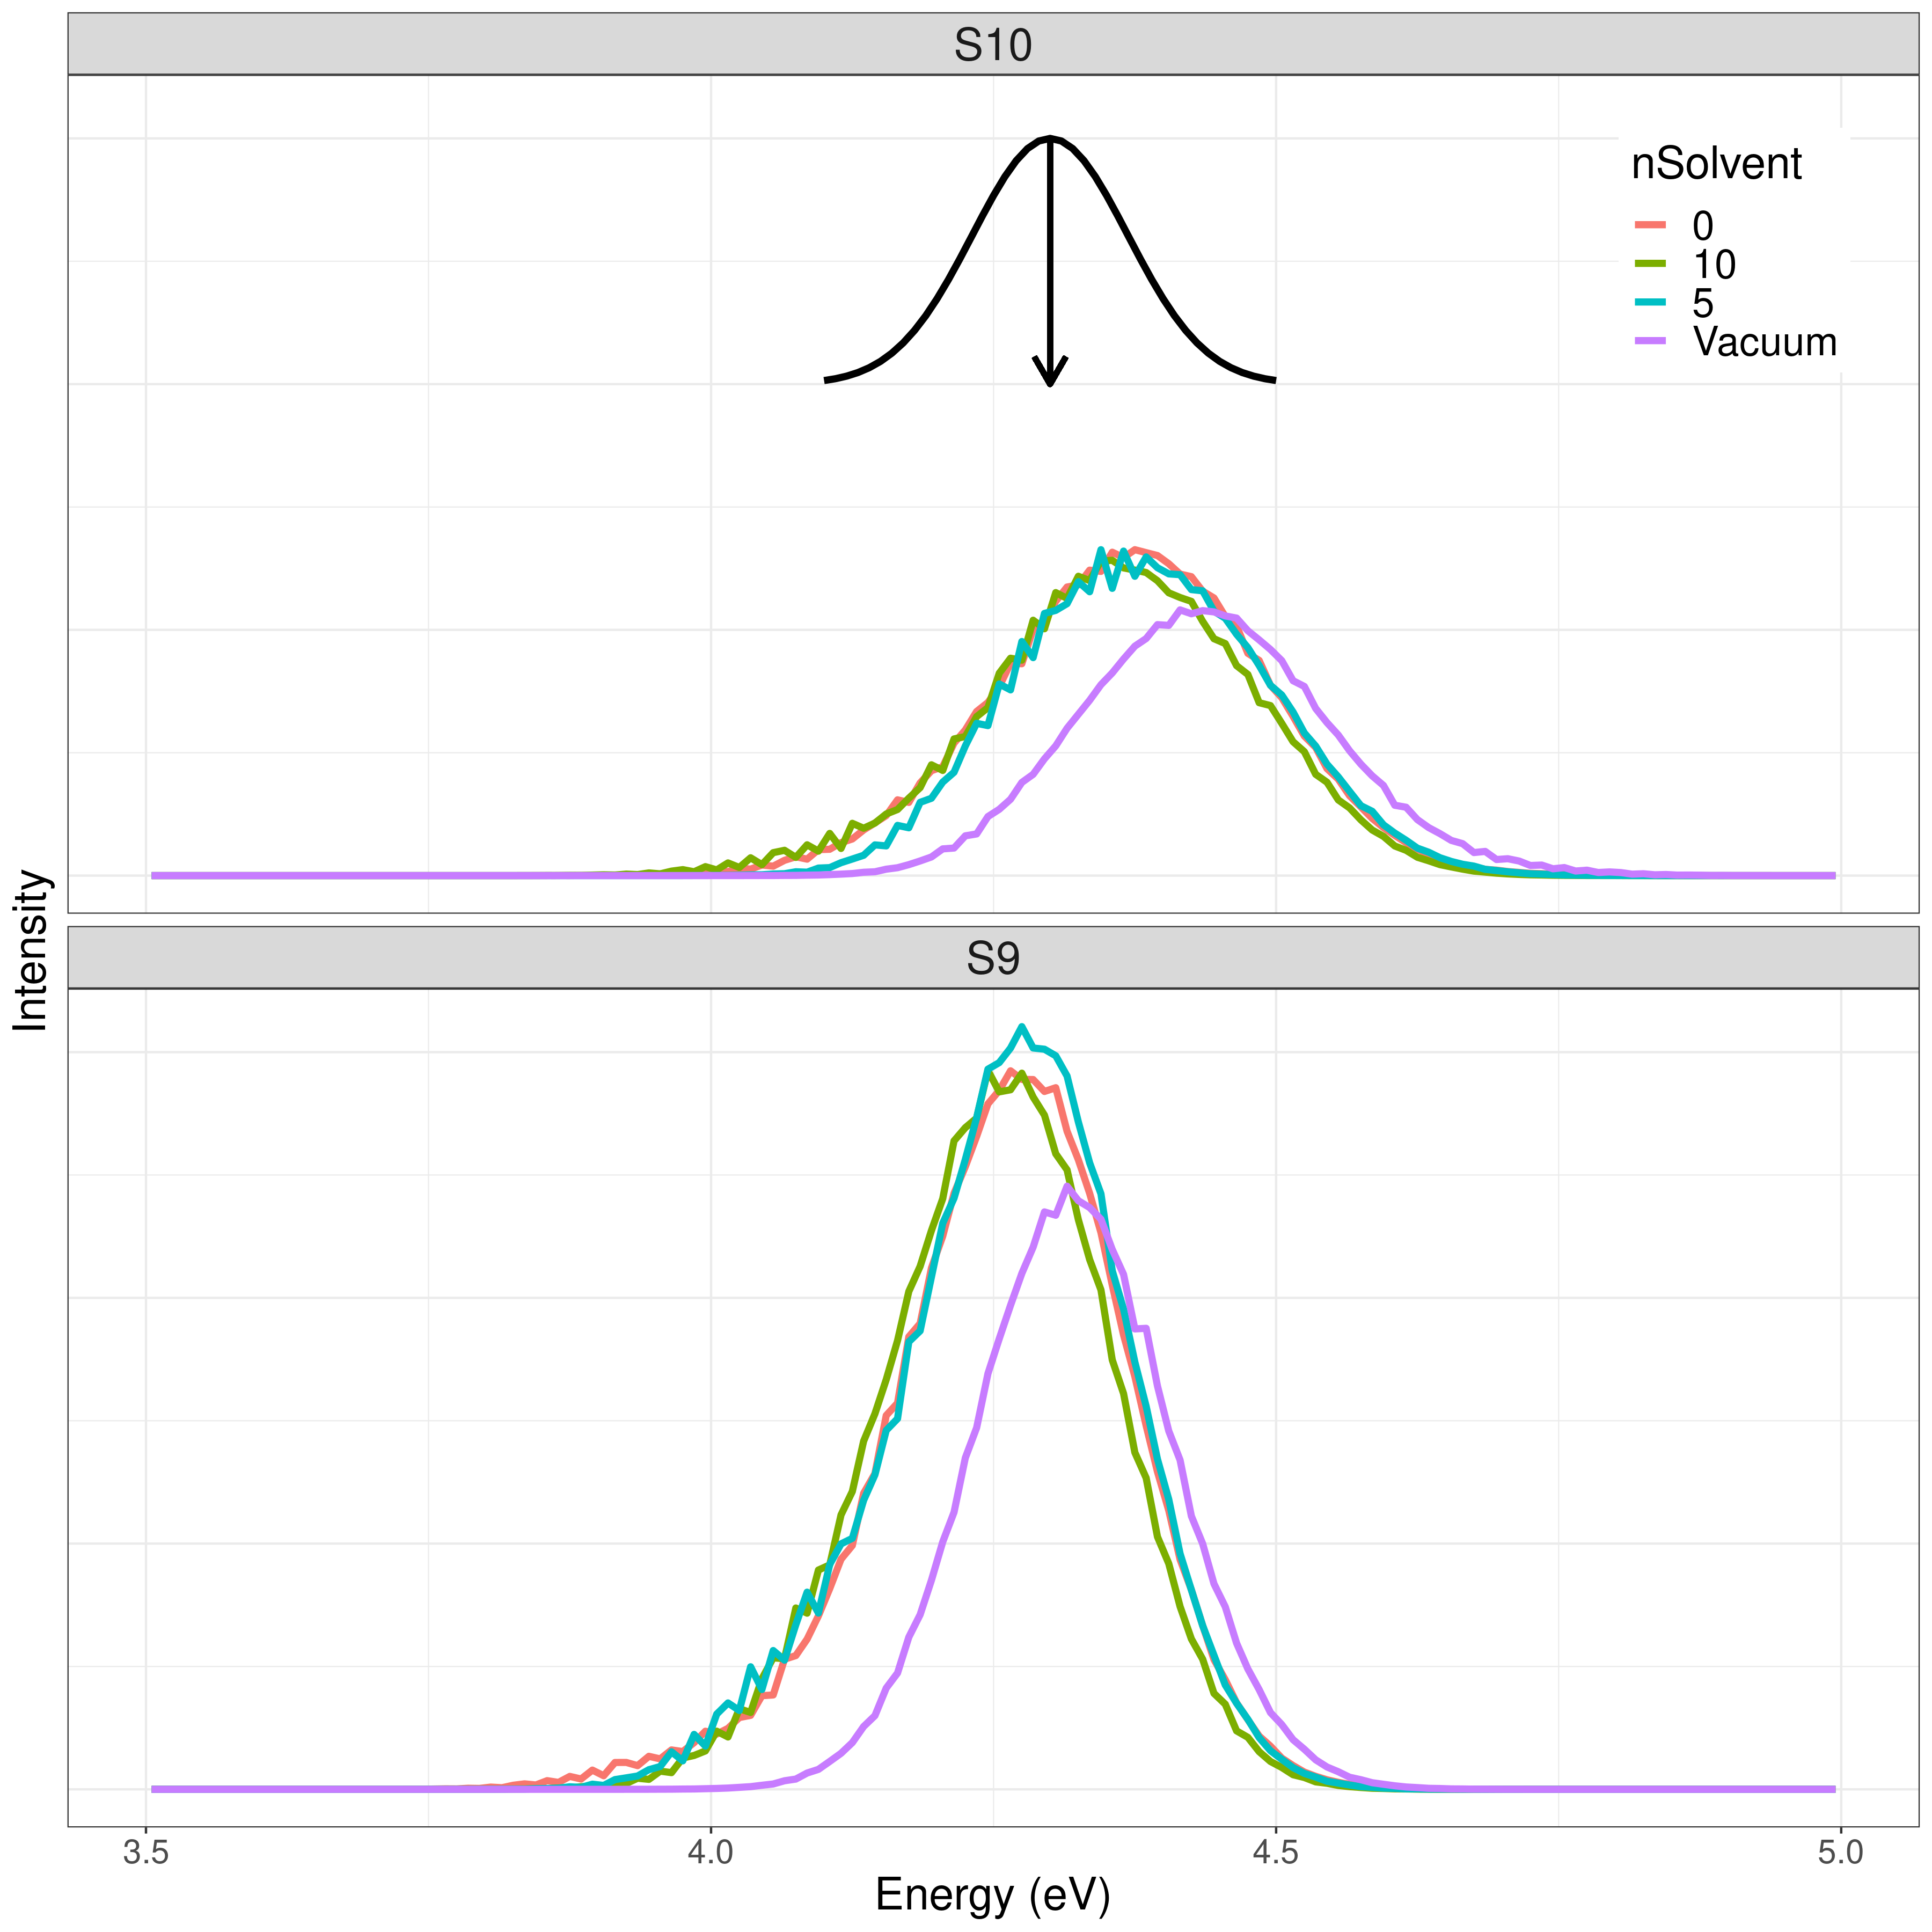
\includegraphics[width=5in]{../Paper2/Images/pulse_pump/spectra.png}
  \captionof{figure}{The calculated absorption spectrum from the first excited state S\(_1\). State energies are differences from the ground state.}
  \label{s1absorption}
\end{minipage}\bigskip

\subsection{State Population Relaxation}

\noindent
\begin{minipage}[c]{\textwidth}
  \centering
  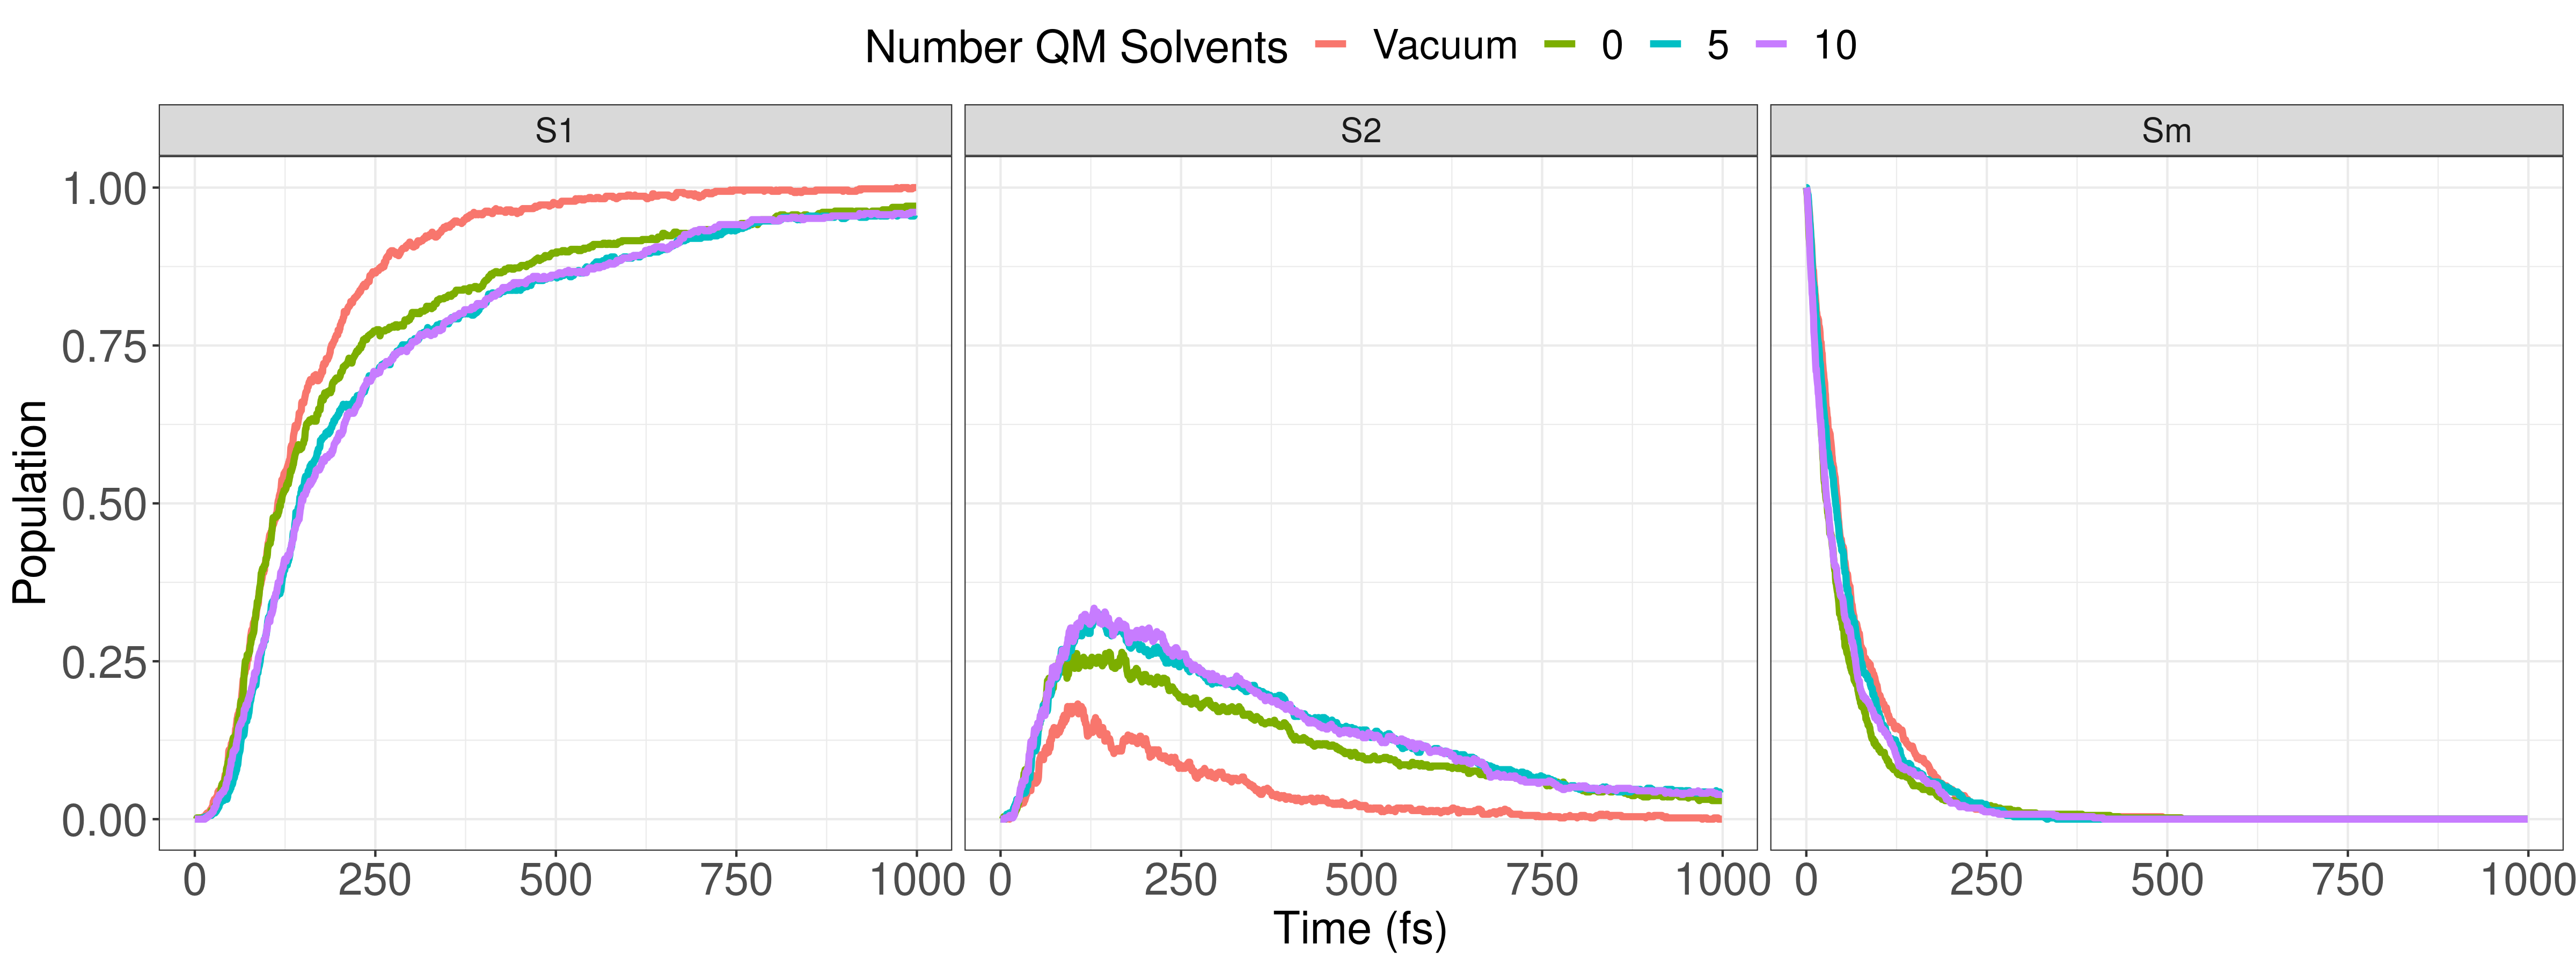
\includegraphics[width=0.9\textwidth]{../Paper2/Images/populations/solvent_comparison.png}
  \captionof{figure}[Test]{Comparison of the population decays or rises of states S\(_1\), S\(_2\), and the initial state S\(_m\) between simulations with varying number of solvents included in the QM region.}
  \label{stateDecay}
\end{minipage}\bigskip

Figure ref:fig:all-populations shows the population of each state calculated as
the number of trajectories at the state's potential energy surface over the
total number of trajectories. S\(_m\) represents the initial state calculated using
the pulse pump calculations previously done. States S\(_7\) and S\(_9\) are included as
the only other "slow" states, or states that reached a population of more than
0.05. The other states were excluded from the graph. These charts show that the
addition of the NO\(_2\) oligimors dramatically speed up the state relaxation. S\(_m\)
ranged from S\(_9\) to S\(_15\) for PPV\(_3\) and S\(_11\) to S\(_21\) for PPV\(_{3}\)-NO\(_{2}\). Figure
ref:fig:s1-populations, shows the rise of the S\(_{1}\) populations over the first
500 fs after excitation. We model these rises by fitting the curves to the
function
\begin{equation}
f(t) = \frac{Ae^{t/\tau}}{A+e^{t/\tau}} - \frac{A}{1+A}
\end{equation}
where $t$ is time, $\tau$ is the relaxation, and $A$ is a constant that
normalizes such that the populations remain between 0 and 1. The results are displayed in ref:table:s1. 
We clearly see that adding a test for trivial-nonavoided crossing slows the rate
of relaxation from a time constant of 258~fs. This is to be expected since we
are now preventing transitions (mostly downward) that should not occur. The
methanol have mixed results with regards to PPV3 and seem to slightly slow the
relaxation of PPV\(_3\)-NO\(_2\). Experiments using ultrafast spectroscopy have shown that
for PPV thin films the time constant for relaxations should be around 200 fs.
However, that was on thin films and for PPV\(_3\), the energy gap !! Average S\(_1\) ->
S\(_m\) energy gap) than in the thin film (0.8eV). Previous research using the
NAESMD framework have shown a time constant of 394 fs, but this was without the
test for trivial non-avoided crossings.

\subsection{Potential Energy Relaxation}

\noindent
\begin{minipage}[c]{\textwidth}
  \centering
  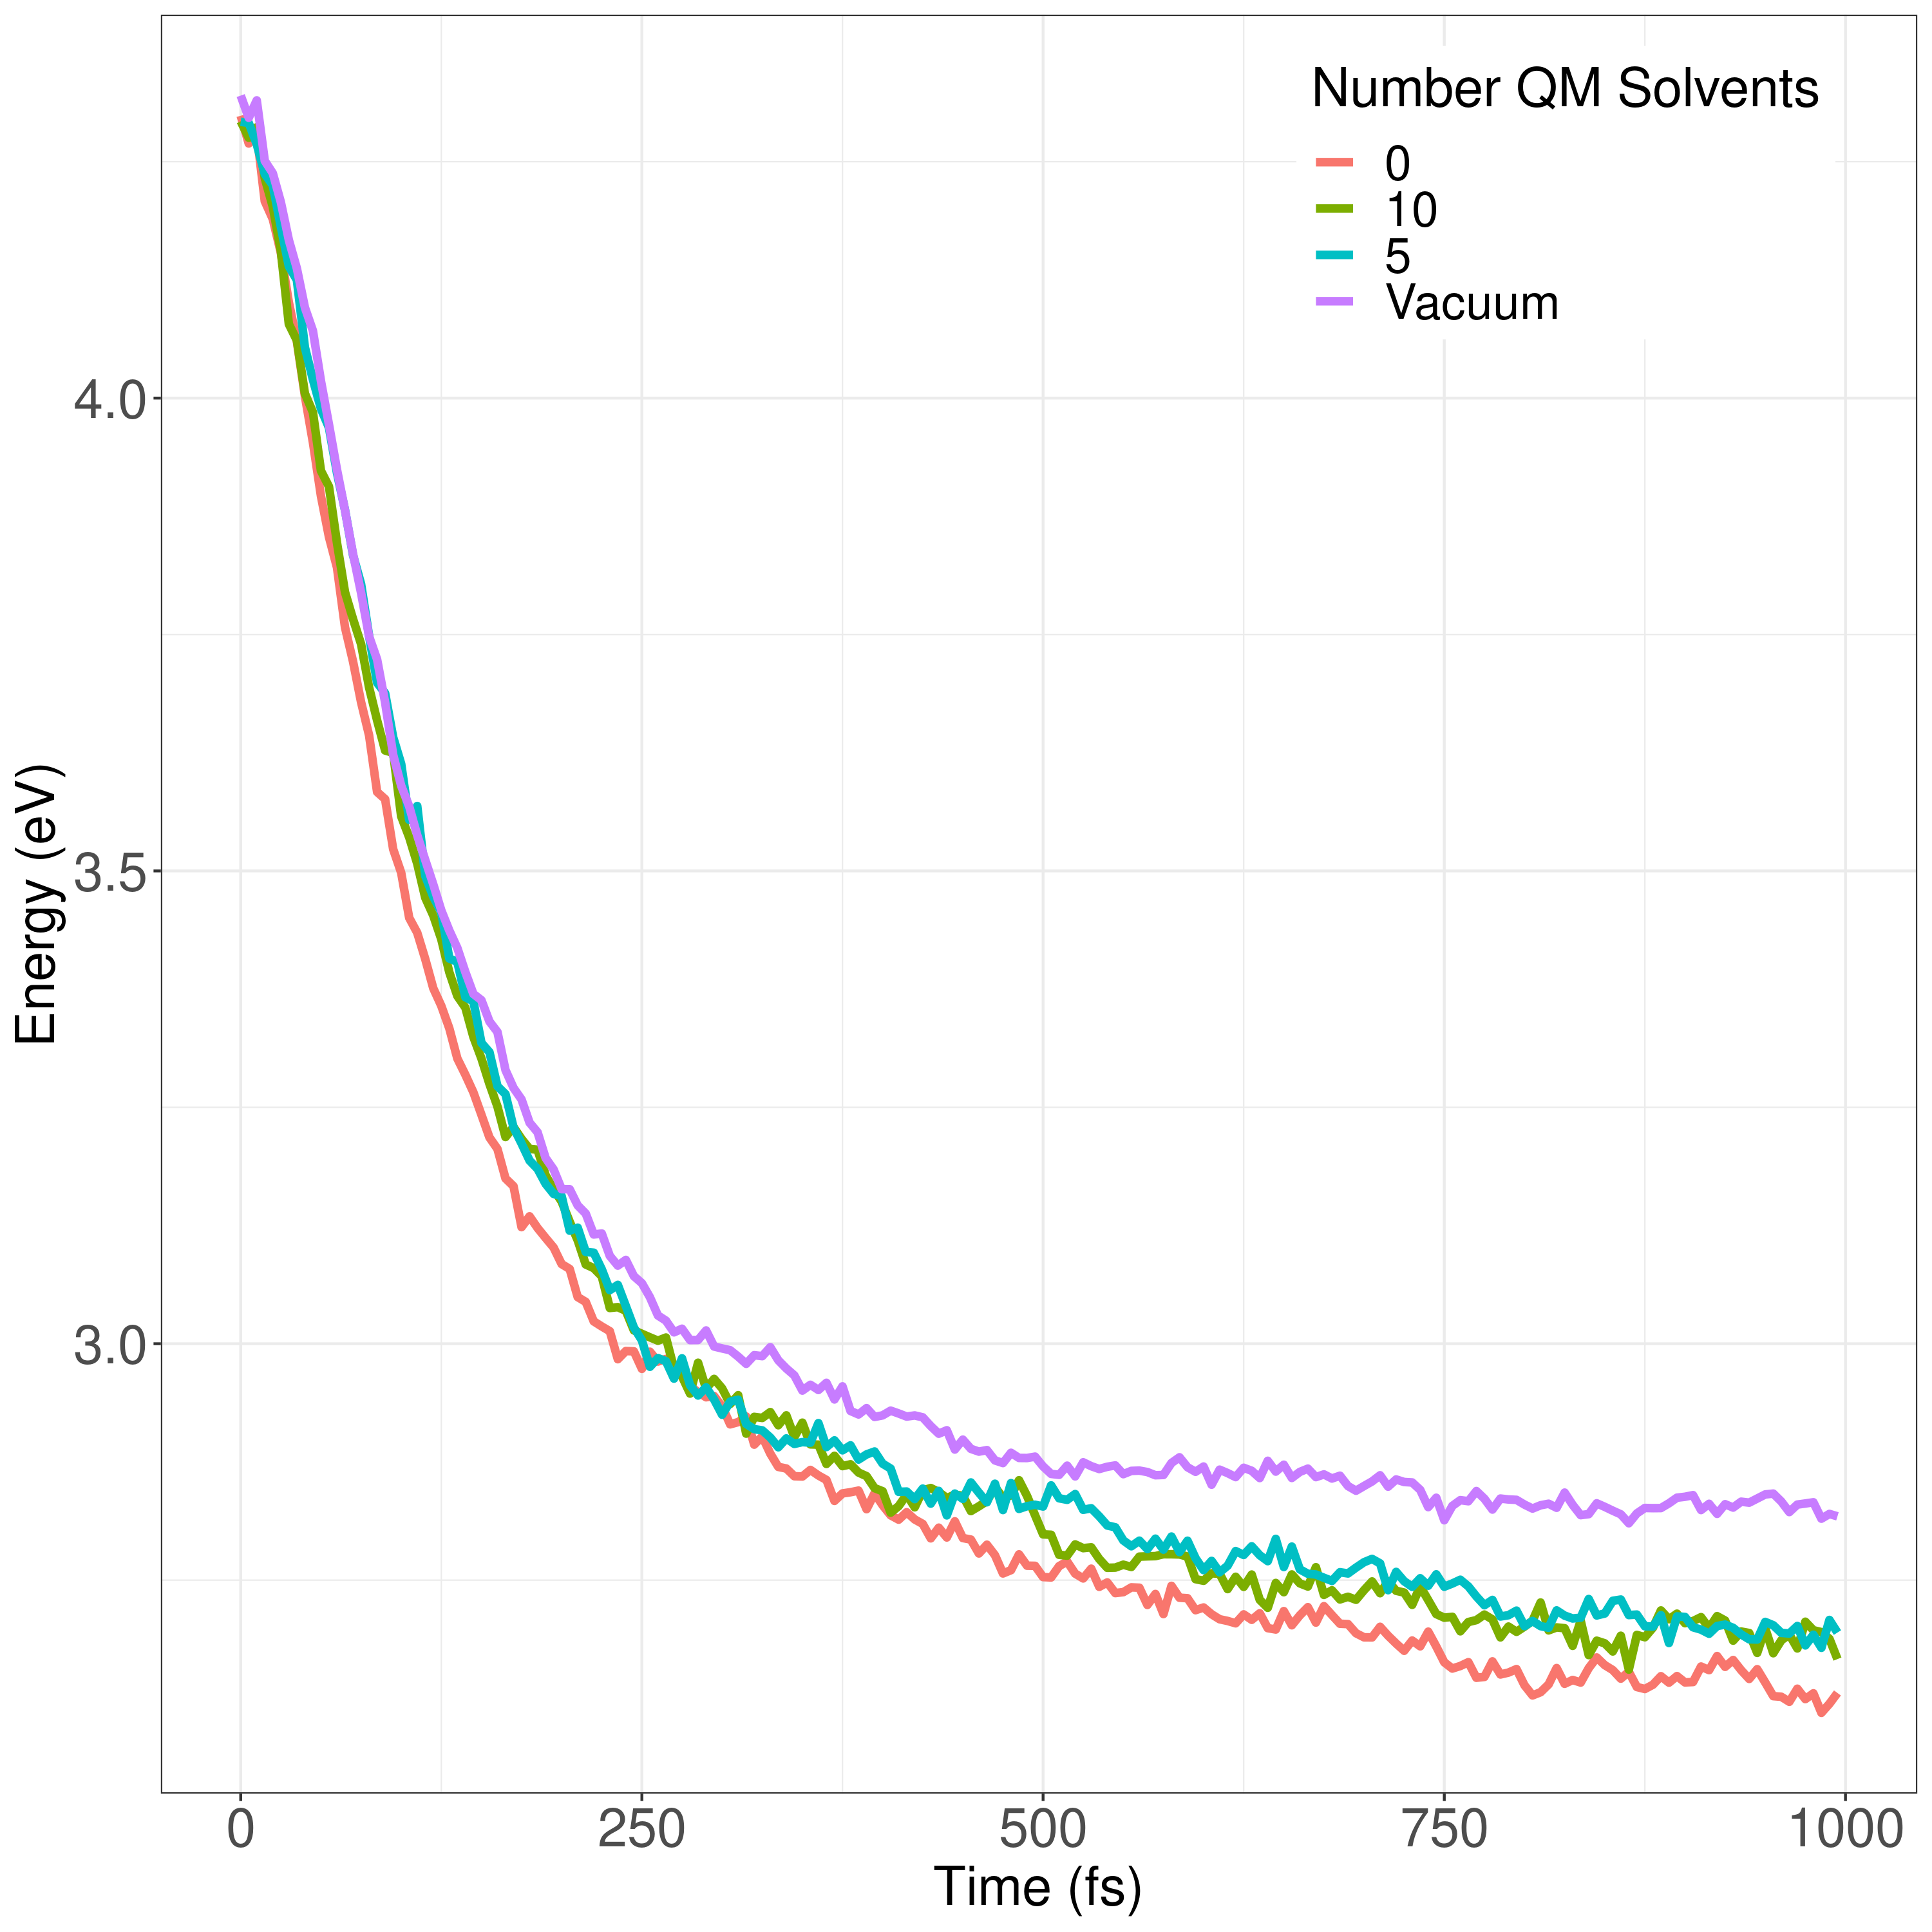
\includegraphics[width=0.5\textwidth]{../Paper2/Images/potential_energies/solvent_comparison.png}
  \captionof{figure}{Potential energy difference from the intial ground state during dynamics averaged over trajectories.}
  \label{}
\end{minipage}\bigskip

\subsection{Bond Length Alternation}

\subsection{Torsional Angle Relaxation}

\noindent
\begin{minipage}[c]{\textwidth}
  \centering
  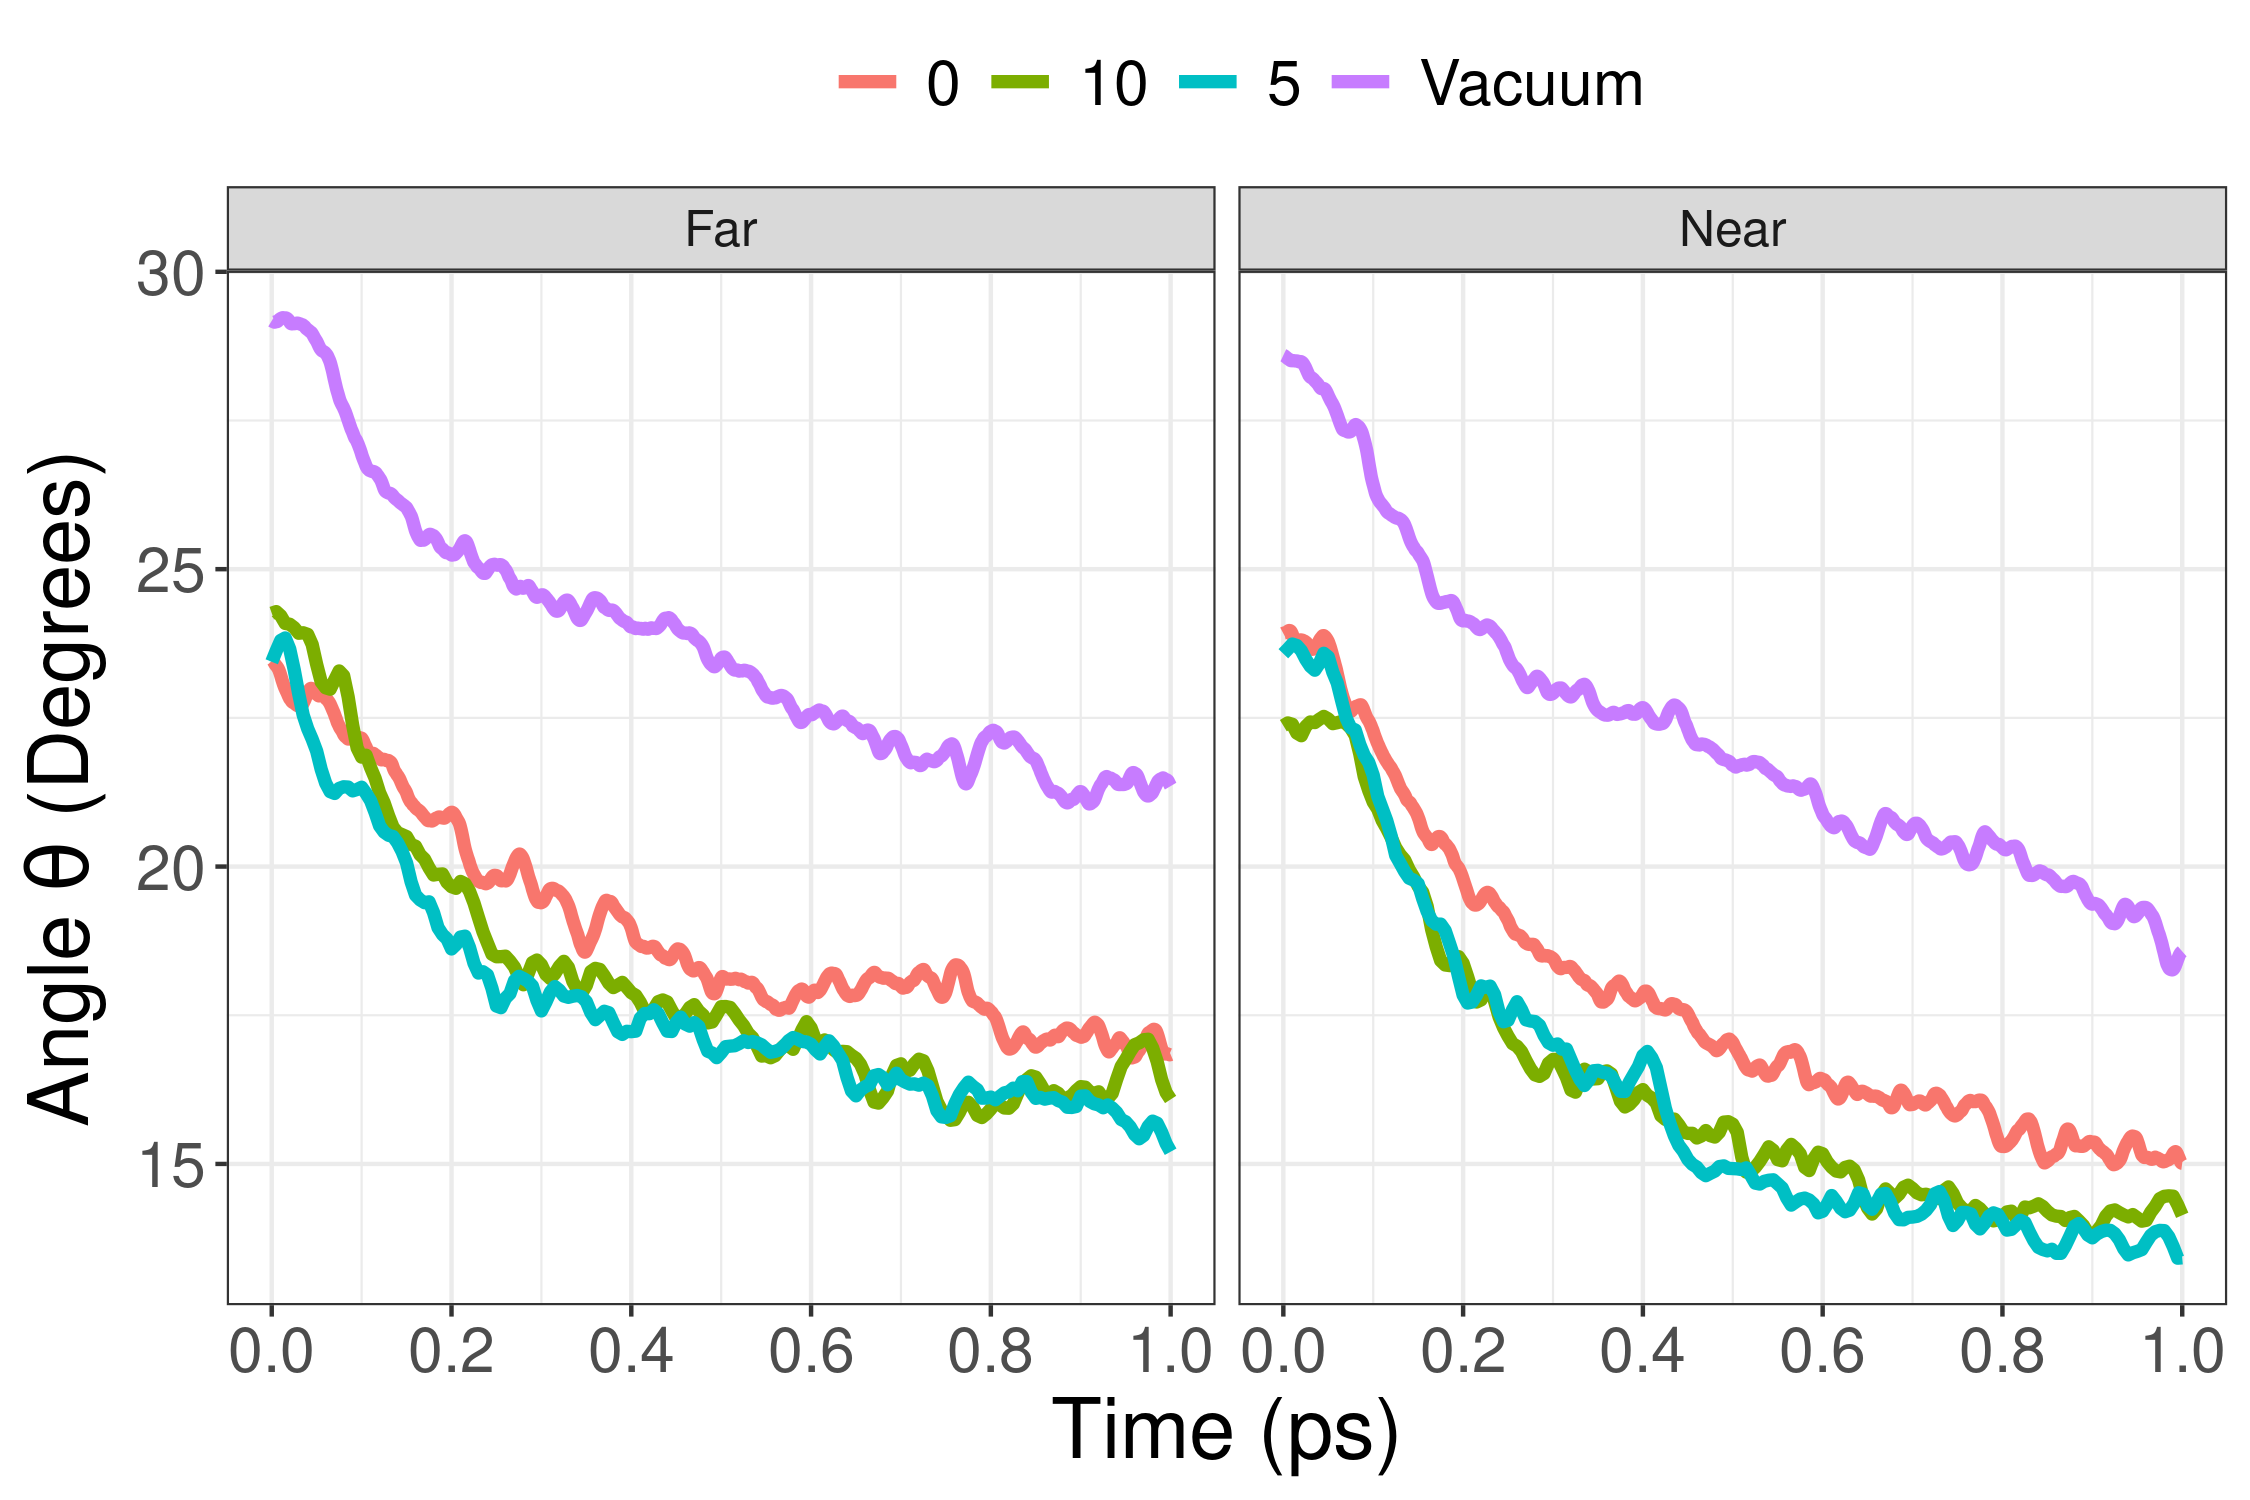
\includegraphics[width=5in]{../Paper2/Images/dihedral/solvent_comparison.png}
  \captionof{figure}{Dihedral angles of PPV\(_{3}\)-NO\(_{2}\) with varying number of solvents included in the QM region.}
  \label{dihedralNonadiabatic}
\end{minipage}\bigskip

\subsection{Widberg Bond Relaxation}

\subsection{Bond Orders}
\noindent
\begin{minipage}[c]{\textwidth}
  \centering
  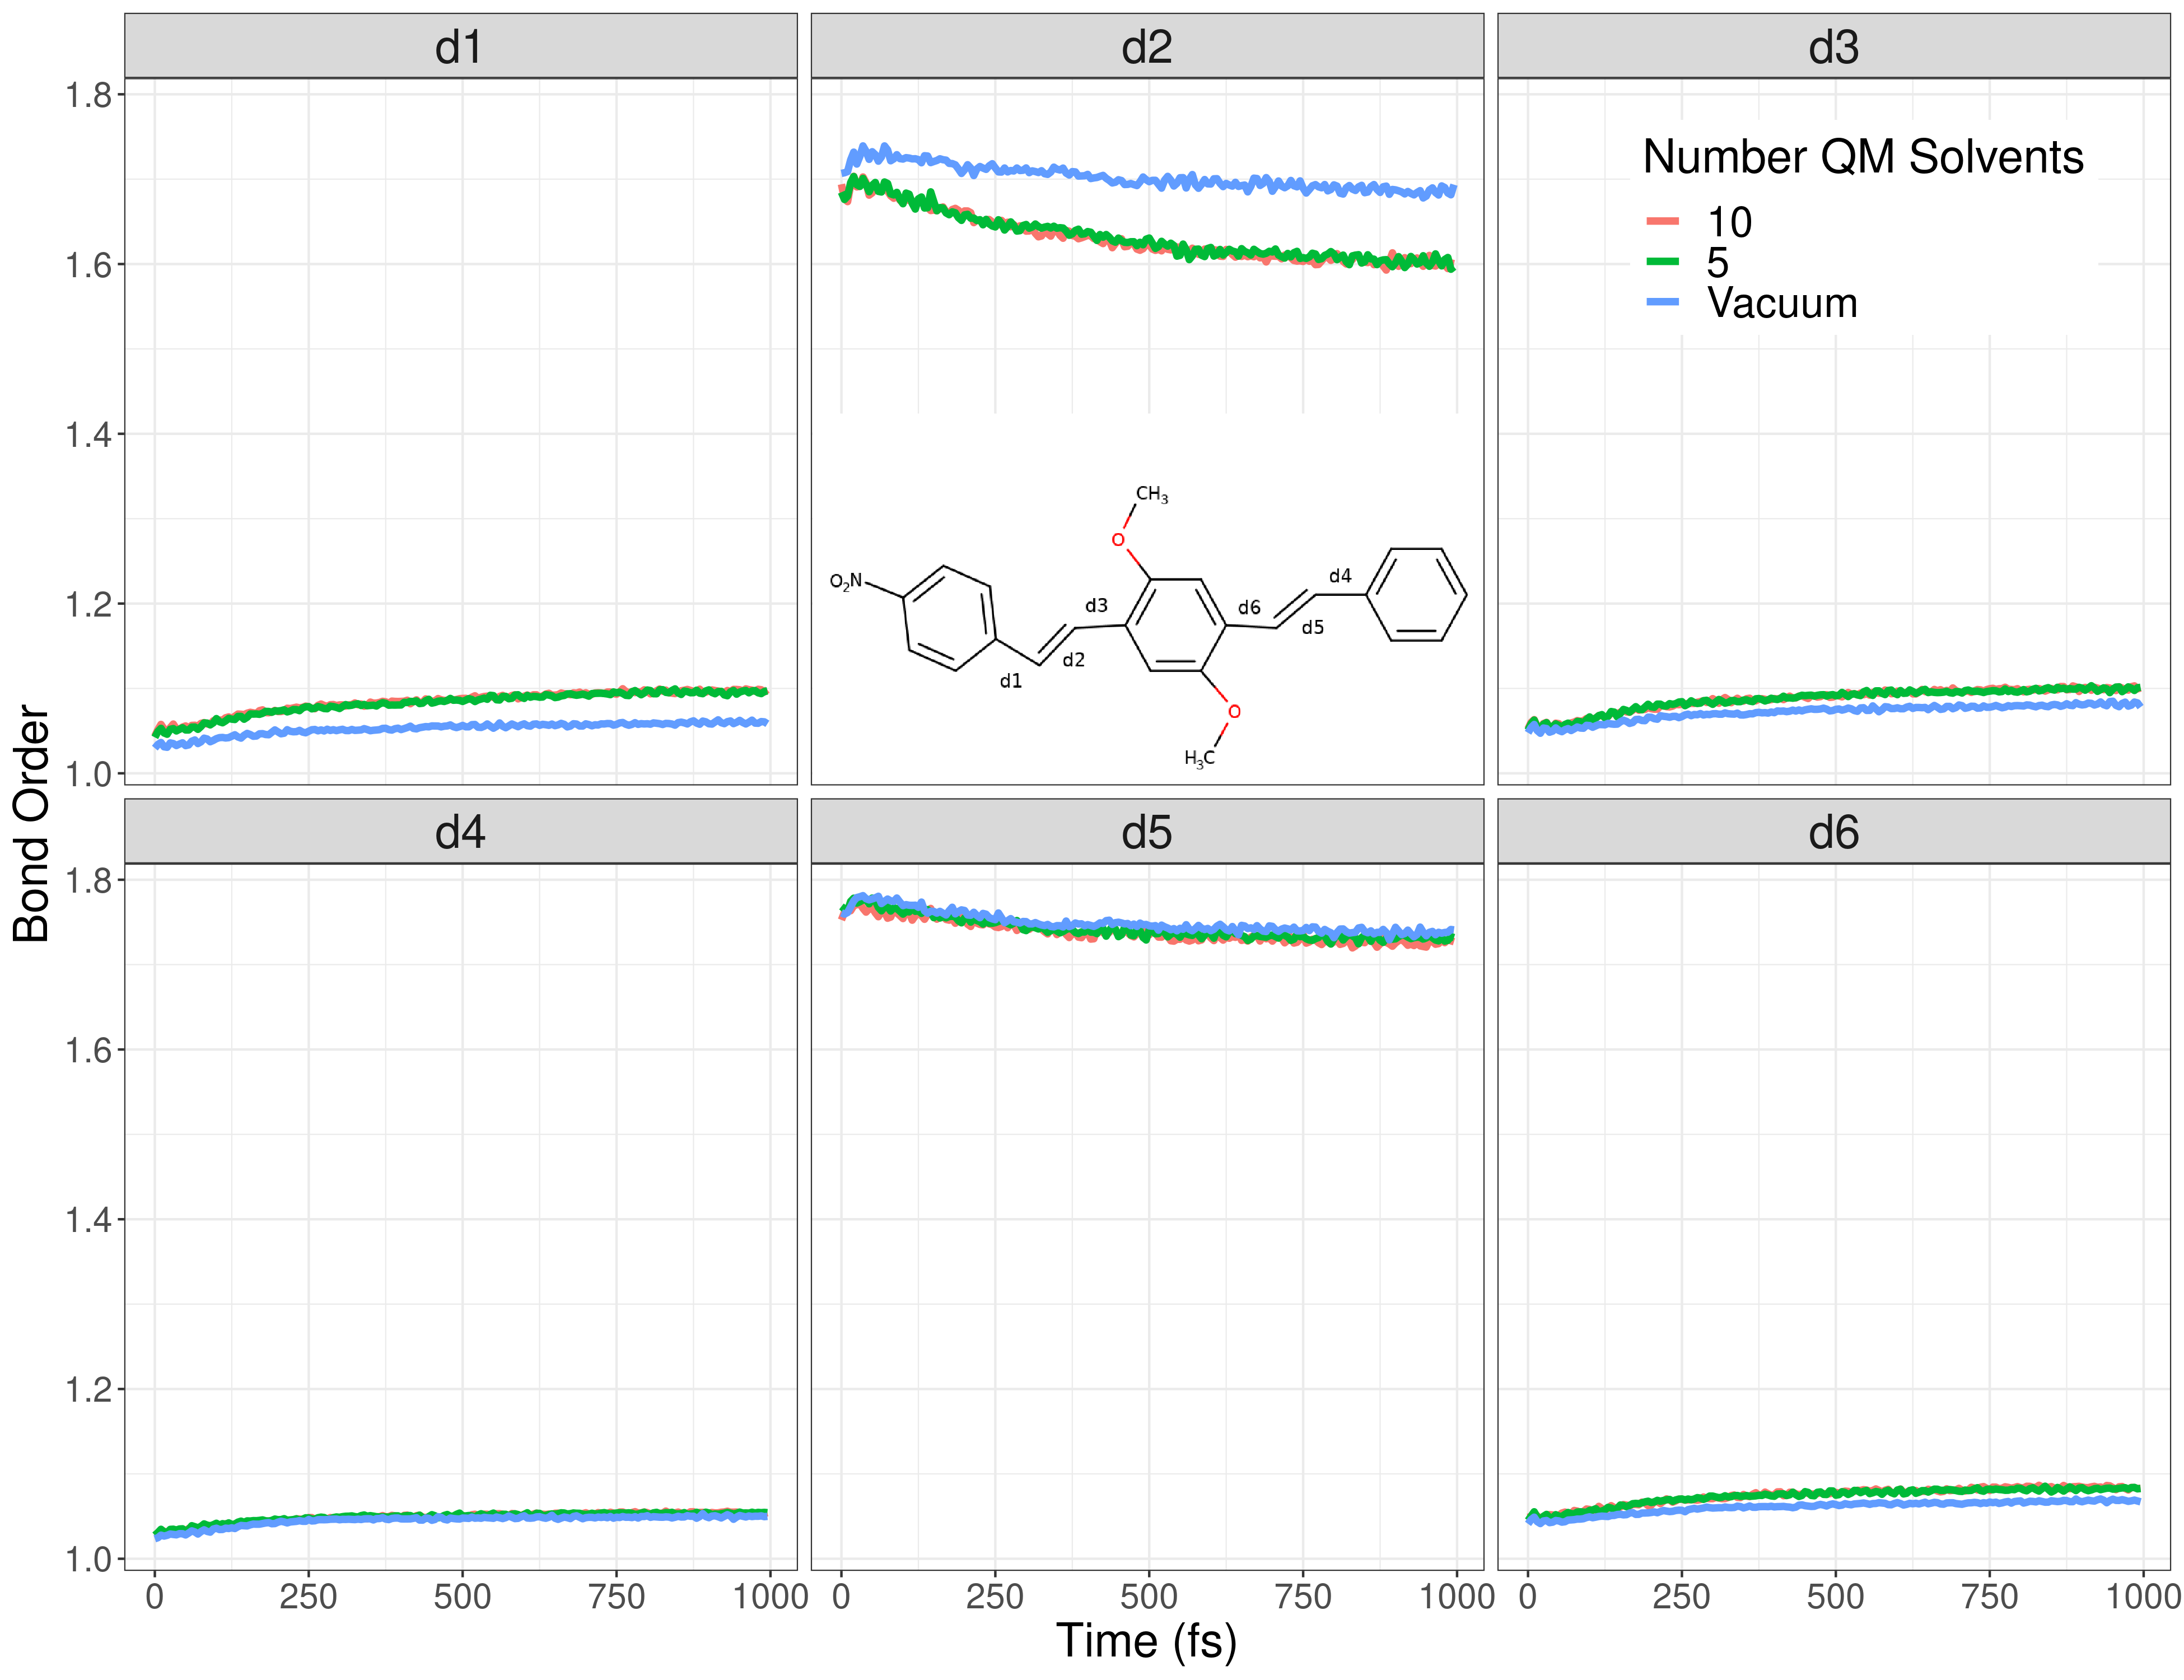
\includegraphics[width=5in]{../Paper2/Images/bond_order/solvent_comparison.png}
  \captionof{figure}[Wiberg Bond Orders in Nonadiabatic Dynamics]{The Wiberg Bond Orders averaged over the ensemble of trajectories for select bonds for PPV\(_3\)-NO\(_2\) with various number of solvents included in the QM region.}
  \label{bondOrderNonadiabatic}
\end{minipage}\bigskip
% Modified from old template.

% \begin{algorithm}% Example showing the weird "algorithm" environment works...
%     \captionof{algorithm}{Test Caption}
% \end{algorithm}
% \addObject{TestStuff!}%     This is probably the command that a normal author will use to add objects.

% \chapter{EXAMPLES OF EDITOR/Author TOOLS, TABLES, AND IMAGES}% Notice that we can use chapter/section etc breaks in the master file if we want, and then use \input instead of \include to avoid unneccessary page breaks.
% \section{Example of using the authorRemark and editorRemark}
If you don't see any blue or red type under this line, then you almost certainly need to include the optional ``editMode" to the document class. Thus your document class (first line) should read \verb|\documentclass[editMode]{ufdissertation}|.

\authorRemark{Test! This is a remark written by the author, to themselves, for review purposes. It will be suppressed unless editMode is used in the class options.}

\editorRemark{This is an editor's remark, written by an editor in-line so that they can write into the content itself with something easy to see. But the remark will be suppressed unless editMode is used in the class options.

To get this remark to go away, simply remove ``editMode" from the documentclass options at the top of the user's tex-file. This also removes the blue Author Remarks.
}%     Stuff about using editorRemark and authorRemark commands
% \section{Table Examples}% Notice that the section command needs to be included in the file somewhere. The \include command will not generate chapter or section breaks automatically.
You may notice that some tables get moved outside of where you placed them. This is because \LaTeX{} is a little too helpful when it comes to placement of `float' types; which includes tables and figures. You can get around this by using the ``H" parameter in the table environment, or the `multiFigure' environment described in the ``adding graphics section"; ie section \ref{Sec:addingGraphics}

\begin{table}[H]
\begin{tabular}{llcr}
Some    & Data  & Goes  & Here\\
Some    & Data  & Goes  & Here\\
Some    & Data  & Goes  & Here\\
Some    & Data  & Goes  & Here\\
\end{tabular}
\caption[An example of a table caption in the incorrect place.]{This table is located in the correct section because it uses the ``H" optional parameter in the table environment, unlike the next tables which have been helpfully moved by \LaTeX{} to the next page, which places them inside the section.

You should also make a note that the caption command is placed after the table itself, which means the caption occurs after the table. The graduate school requires tables to have captions placed {before} the actual table data, so the caption command should be located before the table data. See the next table for an example.}
\end{table}

\begin{table}[]
\caption[A proper table caption location]{Notice that this caption is included above the table data, as per the graduate school requirements. Also note that the caption itself has a short version in the ``List of Tables" which is achieved by using the optional argument of the caption command. See the file source code directly to see the example.

Unfortunately, since we did not use the ``H" parameter in the table environment, this table was placed \textit{after} the next section heading, which is almost certainly not where an author would have wanted it.}
%\begin{center}
\begin{tabularx}{\textwidth}{XXXX}\hline
Some    & Data  & Goes  & Here\\\hline
Some    & Data  & Goes  & Here\\
Some    & Data  & Goes  & Here\\
Some    & Data  & Goes  & Here\\\hline
\end{tabularx}
%\end{center}

\end{table}

\section{Very Long Tables}

There are two approaches to inputting very long tables. You can do it manually, or you can do it using the longtables package. Here we include an example of both. Table \ref{tbl1} is done manually, whereas \ref{tbl2} is done using the longtables package.

\begin{table}[H]
\caption{Feasible triples for highly variable Grid, MLMMH.} \label{tbl1}
\begin{tabularx}{6.5 in}{r l X}
\hline {{Time (s)}} & {{Triple chosen}} & {{Other feasible triples}} \\ \hline
0 & (1, 11, 13725) & (1, 12, 10980), (1, 13, 8235), (2, 2, 0), (3, 1, 0) \\
2745 & (1, 12, 10980) & (1, 13, 8235), (2, 2, 0), (2, 3, 0), (3, 1, 0) \\
5490 & (1, 12, 13725) & (2, 2, 2745), (2, 3, 0), (3, 1, 0) \\
8235 & (1, 12, 16470) & (1, 13, 13725), (2, 2, 2745), (2, 3, 0), (3, 1, 0) \\
10980 & (1, 12, 16470) & (1, 13, 13725), (2, 2, 2745), (2, 3, 0), (3, 1, 0) \\
13725 & (1, 12, 16470) & (1, 13, 13725), (2, 2, 2745), (2, 3, 0), (3, 1, 0) \\
16470 & (1, 13, 16470) & (2, 2, 2745), (2, 3, 0), (3, 1, 0) \\
19215 & (1, 12, 16470) & (1, 13, 13725), (2, 2, 2745), (2, 3, 0), (3, 1, 0) \\
21960 & (1, 12, 16470) & (1, 13, 13725), (2, 2, 2745), (2, 3, 0), (3, 1, 0) \\
24705 & (1, 12, 16470) & (1, 13, 13725), (2, 2, 2745), (2, 3, 0), (3, 1, 0) \\
27450 & (1, 12, 16470) & (1, 13, 13725), (2, 2, 2745), (2, 3, 0), (3, 1, 0) \\
30195 & (2, 2, 2745) & (2, 3, 0), (3, 1, 0) \\
32940 & (1, 13, 16470) & (2, 2, 2745), (2, 3, 0), (3, 1, 0) \\
35685 & (1, 13, 13725) & (2, 2, 2745), (2, 3, 0), (3, 1, 0) \\
38430 & (1, 13, 10980) & (2, 2, 2745), (2, 3, 0), (3, 1, 0) \\
41175 & (1, 12, 13725) & (1, 13, 10980), (2, 2, 2745), (2, 3, 0), (3, 1, 0) \\
43920 & (1, 13, 10980) & (2, 2, 2745), (2, 3, 0), (3, 1, 0) \\
46665 & (2, 2, 2745) & (2, 3, 0), (3, 1, 0) \\
49410 & (2, 2, 2745) & (2, 3, 0), (3, 1, 0) \\
52155 & (1, 12, 16470) & (1, 13, 13725), (2, 2, 2745), (2, 3, 0), (3, 1, 0) \\
54900 & (1, 13, 13725) & (2, 2, 2745), (2, 3, 0), (3, 1, 0) \\
57645 & (1, 13, 13725) & (2, 2, 2745), (2, 3, 0), (3, 1, 0) \\
60390 & (1, 12, 13725) & (2, 2, 2745), (2, 3, 0), (3, 1, 0) \\
63135 & (1, 13, 16470) & (2, 2, 2745), (2, 3, 0), (3, 1, 0) \\
65880 & (1, 13, 16470) & (2, 2, 2745), (2, 3, 0), (3, 1, 0) \\
68625 & (2, 2, 2745) & (2, 3, 0), (3, 1, 0) \\
71370 & (1, 13, 13725) & (2, 2, 2745), (2, 3, 0), (3, 1, 0) \\
74115 & (1, 12, 13725) & (2, 2, 2745), (2, 3, 0), (3, 1, 0) \\
76860 & (1, 13, 13725) & (2, 2, 2745), (2, 3, 0), (3, 1, 0) \\
79605 & (1, 13, 13725) & (2, 2, 2745), (2, 3, 0), (3, 1, 0) \\
82350 & (1, 12, 13725) & (2, 2, 2745), (2, 3, 0), (3, 1, 0) \\
\hline
\end{tabularx}
\end{table}

\begin{table}[h!t!]
\begin{tabularx}{6.5 in}{r l X}
\multicolumn{3}{l}{Table \ref{tbl1}. Continued}\\%
\hline {{Time (s)}} & {{Triple chosen}} & {{Other feasible triples}} \\ \hline
85095 & (1, 12, 13725) & (1, 13, 10980), (2, 2, 2745), (2, 3, 0), (3, 1, 0) \\
87840 & (1, 13, 16470) & (2, 2, 2745), (2, 3, 0), (3, 1, 0) \\
90585 & (1, 13, 16470) & (2, 2, 2745), (2, 3, 0), (3, 1, 0) \\
93330 & (1, 13, 13725) & (2, 2, 2745), (2, 3, 0), (3, 1, 0) \\
96075 & (1, 13, 16470) & (2, 2, 2745), (2, 3, 0), (3, 1, 0) \\
98820 & (1, 13, 16470) & (2, 2, 2745), (2, 3, 0), (3, 1, 0) \\
101565 & (1, 13, 13725) & (2, 2, 2745), (2, 3, 0), (3, 1, 0) \\
104310 & (1, 13, 16470) & (2, 2, 2745), (2, 3, 0), (3, 1, 0) \\
107055 & (1, 13, 13725) & (2, 2, 2745), (2, 3, 0), (3, 1, 0) \\
109800 & (1, 13, 13725) & (2, 2, 2745), (2, 3, 0), (3, 1, 0) \\
112545 & (1, 12, 16470) & (1, 13, 13725), (2, 2, 2745), (2, 3, 0), (3, 1, 0) \\
115290 & (1, 13, 16470) & (2, 2, 2745), (2, 3, 0), (3, 1, 0) \\
118035 & (1, 13, 13725) & (2, 2, 2745), (2, 3, 0), (3, 1, 0) \\
120780 & (1, 13, 16470) & (2, 2, 2745), (2, 3, 0), (3, 1, 0) \\
123525 & (1, 13, 13725) & (2, 2, 2745), (2, 3, 0), (3, 1, 0) \\
126270 & (1, 12, 16470) & (1, 13, 13725), (2, 2, 2745), (2, 3, 0), (3, 1, 0) \\
129015 & (2, 2, 2745) & (2, 3, 0), (3, 1, 0) \\
131760 & (2, 2, 2745) & (2, 3, 0), (3, 1, 0) \\
134505 & (1, 13, 16470) & (2, 2, 2745), (2, 3, 0), (3, 1, 0) \\
137250 & (1, 13, 13725) & (2, 2, 2745), (2, 3, 0), (3, 1, 0) \\
139995 & (2, 2, 2745) & (2, 3, 0), (3, 1, 0) \\
142740 & (2, 2, 2745) & (2, 3, 0), (3, 1, 0) \\
145485 & (1, 12, 16470) & (1, 13, 13725), (2, 2, 2745), (2, 3, 0), (3, 1, 0)\\%
148230 & (2, 2, 2745) & (2, 3, 0), (3, 1, 0) \\
150975 & (1, 13, 16470) & (2, 2, 2745), (2, 3, 0), (3, 1, 0) \\
153720 & (1, 12, 13725) & (2, 2, 2745), (2, 3, 0), (3, 1, 0) \\
156465 & (1, 13, 13725) & (2, 2, 2745), (2, 3, 0), (3, 1, 0) \\
159210 & (1, 13, 13725) & (2, 2, 2745), (2, 3, 0), (3, 1, 0) \\
161955 & (1, 13, 16470) & (2, 2, 2745), (2, 3, 0), (3, 1, 0) \\
164700 & (1, 13, 13725) & (2, 2, 2745), (2, 3, 0), (3, 1, 0) \\
\hline
\end{tabularx}
\end{table}
\newpage

Alternatively, compared to the previous example where we used manual breaks to break the table, we can let LaTeX do this for us, as well as taking care of any recurrent headers and footers, utilizing the \verb|\longtable| command,\footnote{note that the longtable environment is not in a table environment; putting it inside a table environment will stop it from correctly page breaking as needed.} as follows:


\begin{longtable}[h!t!]{p{0.6in}p{1in}p{4.4in}}
    \caption{Duplicate of Previous table, using longtables environment.}\label{tbl2}\\% Default caption at top of table
    \hline {{Time (s)}} & {{Triple chosen}} & {{Other feasible triples}}\\ \hline \endfirsthead% The top row of the first page
    \hline\endfoot%         This line should always be included; it includes a line at the end of the table on every page.
    \caption*{continued} \\% This caption is added to every page after the first as per the \endhead next line.
    \hline{{Time (s)}} & {{Triple chosen}} & {{Other feasible triples}}\\ \hline \endhead%
%                                                               Everything between \endfoot and \endhead here is added at
%                                                                   the top of the table on every page except the first;
%                                                                   The first page is an exception because we have defined a
%                                                                   \endfirsthead row already which superceeds \endhead.
0 & (1, 11, 13725) & (1, 12, 10980), (1, 13, 8235), (2, 2, 0), (3, 1, 0)\\
2745 & (1, 12, 10980) & (1, 13, 8235), (2, 2, 0), (2, 3, 0), (3, 1, 0) \\
5490 & (1, 12, 13725) & (2, 2, 2745), (2, 3, 0), (3, 1, 0) \\
8235 & (1, 12, 16470) & (1, 13, 13725), (2, 2, 2745), (2, 3, 0), (3, 1, 0) \\
10980 & (1, 12, 16470) & (1, 13, 13725), (2, 2, 2745), (2, 3, 0), (3, 1, 0) \\
13725 & (1, 12, 16470) & (1, 13, 13725), (2, 2, 2745), (2, 3, 0), (3, 1, 0) \\
16470 & (1, 13, 16470) & (2, 2, 2745), (2, 3, 0), (3, 1, 0) \\
19215 & (1, 12, 16470) & (1, 13, 13725), (2, 2, 2745), (2, 3, 0), (3, 1, 0) \\
21960 & (1, 12, 16470) & (1, 13, 13725), (2, 2, 2745), (2, 3, 0), (3, 1, 0) \\
24705 & (1, 12, 16470) & (1, 13, 13725), (2, 2, 2745), (2, 3, 0), (3, 1, 0) \\
27450 & (1, 12, 16470) & (1, 13, 13725), (2, 2, 2745), (2, 3, 0), (3, 1, 0) \\
30195 & (2, 2, 2745) & (2, 3, 0), (3, 1, 0) \\
32940 & (1, 13, 16470) & (2, 2, 2745), (2, 3, 0), (3, 1, 0) \\
35685 & (1, 13, 13725) & (2, 2, 2745), (2, 3, 0), (3, 1, 0) \\
38430 & (1, 13, 10980) & (2, 2, 2745), (2, 3, 0), (3, 1, 0) \\
41175 & (1, 12, 13725) & (1, 13, 10980), (2, 2, 2745), (2, 3, 0), (3, 1, 0) \\
43920 & (1, 13, 10980) & (2, 2, 2745), (2, 3, 0), (3, 1, 0) \\
46665 & (2, 2, 2745) & (2, 3, 0), (3, 1, 0) \\
49410 & (2, 2, 2745) & (2, 3, 0), (3, 1, 0) \\
52155 & (1, 12, 16470) & (1, 13, 13725), (2, 2, 2745), (2, 3, 0), (3, 1, 0) \\
54900 & (1, 13, 13725) & (2, 2, 2745), (2, 3, 0), (3, 1, 0) \\
57645 & (1, 13, 13725) & (2, 2, 2745), (2, 3, 0), (3, 1, 0) \\
60390 & (1, 12, 13725) & (2, 2, 2745), (2, 3, 0), (3, 1, 0) \\
63135 & (1, 13, 16470) & (2, 2, 2745), (2, 3, 0), (3, 1, 0) \\
65880 & (1, 13, 16470) & (2, 2, 2745), (2, 3, 0), (3, 1, 0) \\
68625 & (2, 2, 2745) & (2, 3, 0), (3, 1, 0) \\
71370 & (1, 13, 13725) & (2, 2, 2745), (2, 3, 0), (3, 1, 0) \\
74115 & (1, 12, 13725) & (2, 2, 2745), (2, 3, 0), (3, 1, 0) \\
76860 & (1, 13, 13725) & (2, 2, 2745), (2, 3, 0), (3, 1, 0) \\
79605 & (1, 13, 13725) & (2, 2, 2745), (2, 3, 0), (3, 1, 0) \\
82350 & (1, 12, 13725) & (2, 2, 2745), (2, 3, 0), (3, 1, 0) \\
85095 & (1, 12, 13725) & (1, 13, 10980), (2, 2, 2745), (2, 3, 0), (3, 1, 0) \\
87840 & (1, 13, 16470) & (2, 2, 2745), (2, 3, 0), (3, 1, 0) \\
90585 & (1, 13, 16470) & (2, 2, 2745), (2, 3, 0), (3, 1, 0) \\
93330 & (1, 13, 13725) & (2, 2, 2745), (2, 3, 0), (3, 1, 0) \\
96075 & (1, 13, 16470) & (2, 2, 2745), (2, 3, 0), (3, 1, 0) \\
98820 & (1, 13, 16470) & (2, 2, 2745), (2, 3, 0), (3, 1, 0) \\
101565 & (1, 13, 13725) & (2, 2, 2745), (2, 3, 0), (3, 1, 0) \\
104310 & (1, 13, 16470) & (2, 2, 2745), (2, 3, 0), (3, 1, 0) \\
107055 & (1, 13, 13725) & (2, 2, 2745), (2, 3, 0), (3, 1, 0) \\
109800 & (1, 13, 13725) & (2, 2, 2745), (2, 3, 0), (3, 1, 0) \\
112545 & (1, 12, 16470) & (1, 13, 13725), (2, 2, 2745), (2, 3, 0), (3, 1, 0) \\
115290 & (1, 13, 16470) & (2, 2, 2745), (2, 3, 0), (3, 1, 0) \\
118035 & (1, 13, 13725) & (2, 2, 2745), (2, 3, 0), (3, 1, 0) \\
120780 & (1, 13, 16470) & (2, 2, 2745), (2, 3, 0), (3, 1, 0) \\
123525 & (1, 13, 13725) & (2, 2, 2745), (2, 3, 0), (3, 1, 0) \\
126270 & (1, 12, 16470) & (1, 13, 13725), (2, 2, 2745), (2, 3, 0), (3, 1, 0) \\
129015 & (2, 2, 2745) & (2, 3, 0), (3, 1, 0) \\
131760 & (2, 2, 2745) & (2, 3, 0), (3, 1, 0) \\
134505 & (1, 13, 16470) & (2, 2, 2745), (2, 3, 0), (3, 1, 0) \\
137250 & (1, 13, 13725) & (2, 2, 2745), (2, 3, 0), (3, 1, 0) \\
139995 & (2, 2, 2745) & (2, 3, 0), (3, 1, 0) \\
142740 & (2, 2, 2745) & (2, 3, 0), (3, 1, 0) \\
145485 & (1, 12, 16470) & (1, 13, 13725), (2, 2, 2745), (2, 3, 0), (3, 1, 0)\\%
148230 & (2, 2, 2745) & (2, 3, 0), (3, 1, 0) \\
150975 & (1, 13, 16470) & (2, 2, 2745), (2, 3, 0), (3, 1, 0) \\
153720 & (1, 12, 13725) & (2, 2, 2745), (2, 3, 0), (3, 1, 0) \\
\newpage% Force a pagebreak here so that we don't have a stranded row.
156465 & (1, 13, 13725) & (2, 2, 2745), (2, 3, 0), (3, 1, 0) \\
159210 & (1, 13, 13725) & (2, 2, 2745), (2, 3, 0), (3, 1, 0) \\
161955 & (1, 13, 16470) & (2, 2, 2745), (2, 3, 0), (3, 1, 0) \\
164700 & (1, 13, 13725) & (2, 2, 2745), (2, 3, 0), (3, 1, 0) \\
\end{longtable}

%    Stuff about using Tables.
% \section{Examples of Adding Graphics}
\label{Sec:addingGraphics}
All of the below code with subfigures A-Z was generated with:
\begin{verbatim}
\begin{multiFigure}
\addFigure{0.3}{./theworld.png}
\addFigure{0.2}{./theworld.png}
\addFigure{0.4}{./theworld.png}
\addFigure[Z]{0.6}{./theworld.png}
\captionof{figure}[This is a test caption.]{This is a test caption. 
This text has the bit for the whole figure. 
Meanwhile, subfigure A is weird looking map. 
Subfigure B is a smaller map. 
And Subfigure C is a bigger but still weird looking map. 
Moreover, I can override the map, which is why Z is 
another weird map that came after map C.}
\end{multiFigure}
\end{verbatim}
Note that \LaTeX{} can be pretty fickle when it comes to placing figures relative to text near the figure. Specifically, the ``Figure" environment is a `float' type, which is placed somewhere ``nearby" where it appears in the text, which can be pretty frustrating. For this reason I have circumvented the `float' part of the figure in order to allow more control over the figure placement. So if one uses the \verb|\begin{figure}\end{figure}| construction, the figure may appear in a slightly weird place, whereas you can use the \verb|\begin{multiFigure}\end{multiFigure}| even with only 1 figure, to force placement to work. The only caveat here is that captions need to be placed using the command \verb|\captionof{<NAME>}[<LIST-ENTRY>]{<CAPTION>}| where NAME is the type of caption, LIST-ENTRY is what appears in the `List of' at the beginning of the thesis, and CAPTION is the actual caption.

\begin{multiFigure}
\addFigure{0.3}{./theworld.png}
\addFigure{0.2}{./theworld.png}
\addFigure{0.4}{./theworld.png}
\addFigure[Z]{0.6}{./theworld.png}
\captionof{figure}[This is a test caption.]{This is a test caption. This text has the bit for the whole figure. Meanwhile, subfigure A is weird looking map. Subfigure B is a smaller map. And Subfigure C is a bigger but still weird looking map. Moreover, I can override the map, which is why Z is another weird map that came after map C.}
\end{multiFigure}

\begin{multiFigure}
\addFigure{0.9}{./theworld.png}
\captionof{figure}{This is a super-long caption to make sure that the caption in the list-of section is correctly single space with the blank white line between captions. That being said, you should probably always use the list-entry optional argument in the captionof command to write a shorter caption instead of this nonsense.}
\end{multiFigure}

\section{A Note On Graphics}
The command \verb|\addFigure| in the multiFigure environment, and/or the command \verb|\includegraphics| will take almost every type of graphic file currently in use as of the writing of this template. The only notable exception is the bitmap, ie .bmp file. Most software won't save to bitmap without specifically requesting it at this point, but if you have generated a .bmp file you can load it in most any graphic editor (eg MSpaint or photoshop) and save it as a different file type, such as .PNG which is significantly smaller file size as well. Note that the commands typically require the file extension to be included, and it is case sensitive. Thus in the above \verb|\addFigure{0.2}{./theworld.png}| works but \verb|\addFigure{0.2}{./theworld.PNG}| would error and \verb|\addFigure{0.2}{./theworld}| may or may not work depending on which specific TeX editor you are using.

%    Stuff about using Images.

\end{document}
